\documentclass[a4paper,12pt,oneside,spanish]{book}
\usepackage[utf8]{inputenc}
\usepackage{graphicx}
\usepackage{rotating}
\usepackage{paralist}
\usepackage{enumitem}
\usepackage[spanish]{babel}
\usepackage{geometry}
\usepackage{float}
\usepackage{hyperref}
\usepackage{kantlipsum,setspace}
\usepackage[center]{caption}
\usepackage{unicode}
\usepackage{collcell}
\usepackage{rotating}
\usepackage{csquotes}
\usepackage{multirow,fixltx2e}
\usepackage{booktabs}
\usepackage{titlesec}
\usepackage{color}
\usepackage[table]{xcolor}
\usepackage{setspace}
\usepackage[nottoc,notlot,notlof]{tocbibind}
\usepackage{stackengine}
\newcommand\xrowht[2][0]{\addstackgap[.5\dimexpr#2\relax]{\vphantom{#1}}}

\captionsetup[figure]{font={stretch=0.2}} 
\captionsetup[figure]{font={footnotesize}}
 
\hypersetup{
	colorlinks=true,
	linkcolor=black,
	filecolor=magenta,      
	urlcolor=cyan,
}

\setlength{\paperwidth}{21,0cm}          
\setlength{\paperheight}{29,7cm}       
\setlength{\textwidth}{16.3cm}         
\setlength{\textheight}{23.7cm}        
\setlength{\topmargin}{-0.8cm}     

\usepackage{fancyhdr}
\fancypagestyle{plain}{\fancyfoot[C]{\scriptsize Universidad Católica Campus Itapúa. Ingeniería Informática.}}
\pagestyle{plain}  

\fancyhead[L]{\fontsize{10}{12}}
\pagestyle{fancy}     
\lhead{\scriptsize Entrenamiento de redes neuronales para la detección\\ en tiempo real de amenazas y agresiones humanas en imágenes secuenciales}
\rhead{\thepage}

\setlength{\oddsidemargin}{0.25cm}   
\setlength{\evensidemargin}{0.20cm} 
\renewcommand{\baselinestretch}{1.2}
\renewcommand{\footrulewidth}{0.4pt}% default is 0pt

\tolerance=1
\emergencystretch=\maxdimen
\hyphenpenalty=10000
\hbadness=10000

\makeatletter
\def\@makechapterhead#1{%
	{\parindent \z@ \raggedright \normalfont
		\vskip 1\p@
		\interlinepenalty\@M
		\Huge \bfseries #1\par\nobreak
		\vskip 15\p@
}}
\def\@makeschapterhead#1{%
	{\parindent \z@ \raggedright
		\normalfont
		\interlinepenalty\@M
		\Huge \bfseries  #1\par\nobreak
		\vskip 15\p@
}}
\makeatother

\begin{document}
\thispagestyle{empty}
\begin{figure}[h!]
	
\includegraphics[width=100pt]{Imagenes/logo.png}
	\centering
\end{figure}
\vspace*{0.1cm}
\begin{center}
	{\LARGE {Universidad Católica ``Nuestra Señora de la Asunción'' Campus Itapúa}}
\end{center}
\vspace*{0.1cm}
\begin{center}
	{\large \rm \textbf {Facultad de Ciencias y Tecnologías}}
\end{center}
\vspace*{0.1cm}
\begin{center}
	{\large \rm \textbf {Carrera de Ingeniería Informática}}
\end{center}	
\vspace*{0.2cm}
\begin{center}
	{\large \rm \textbf {Tesis de grado}}
\end{center}
	
\baselineskip 30pt
\vspace*{1cm}
\begin{center}
	{\large \rm Entrenamiento de redes neuronales para la detección en tiempo real de amenazas y agresiones humanas en imágenes secuenciales}
\end{center}

\vspace*{1cm}

\begin{center}
	{\sc  Gustavo Enrique Escobar Krug\\}
	\vspace*{0.1cm}
	
	\center{Docente tutor:}  
	\center{Exp. Nidia Gagliardi}
\end{center}
\vspace*{2cm}
\begin{center}
	{\large \rm 2019}
\end{center}


\spacing{1.5}


%%%%%%%%%%%%%%%%%%%%%%%%%%%%%%%%%%%%%%%%%%%%%%%%%%%%%%%%%%%%%%%%%%%%%%%%%%%%%%
\newpage
\clearpage
\thispagestyle{fancy}
\setcounter{page}{1}
\pagenumbering{arabic}
\setlength{\parskip}{1.3em}
\begin{flushright}
	\subsection*{Dedicatoria}
	A mis abuelos, \\
	donde quiera que estén.
\end{flushright}

\newpage
\begin{flushright}
	\subsection*{Agradecimientos}
	A toda mi familia, \\
	que supo ayudarme y apoyarme \\
	en tiempos difíciles. \\
	Mi deuda con ustedes es inmensa.\par
	
	A mi tutora por los años de dedicación\\
	y comprensión que tuvo hacia mi.\\
	Es un ejemplo a seguir.\\
	
\end{flushright}

\newpage
\tableofcontents

\newpage
\listoffigures

\newpage
\clearpage
\thispagestyle{fancy}
\setlength{\parskip}{1.3em}
\chapter{Resumen}
El propósito del siguiente trabajo de tesis es el de desarrollar una solución aplicativa capaz de detectar una actividad delictiva expresada a través de poses humanas captadas por cámaras de video en tiempo real, emitiendo alertas, visual y sonora. \par 

La idea surge a partir de la observación de numerosos hechos delictivos en donde el ataque o agresión, con o sin armas, logra reducir y neutralizar a las víctimas sin que puedan solicitar ayuda.\par 

Para el desarrollo de la solución se pusieron en práctica conceptos de inteligencia artificial y se utilizaron herramientas de Inteligencia Artificial para la detección de actividad humana delictiva en secuencias de video.\par 

Palabras clave: \textit{Pose, Delictiva, Inteligencia Artificial, Redes neuronales, Entrenamiento, Detección}.

\newpage
\clearpage
\thispagestyle{fancy}
\setlength{\parskip}{1.3em}
\chapter{Abstract}
The purpose of the following thesis work is to develop an application solution capable of detecting a criminal activity expressed through human poses captured by video cameras in real time, emitting alerts, visual and sound. \par

The idea arises from the observation of numerous criminal acts in which the attack or aggression, with or without weapons, manages to reduce and neutralize the victims without being able to request help.\par

For the development of the solution, artificial intelligence concepts were put into practice and Machine Learning tools were used to detect human criminal activity in video sequences.\par

Keywords: \textit {Pose, Criminal, Artificial Intelligence, Neural Networks, Training, Detection}.

\newpage
\setlength{\parskip}{0.8em}
\chapter{Introducción} 
\section{Planteamiento General}
La delincuencia es un mal en crecimiento que afecta a toda sociedad sin importar el estrato social de la víctima, a quien, en muchas ocasiones, el perjuicio puede suponer la pérdida parcial o completa de sus bienes de alto valor, o incluso hasta la vida.\par 
 
Numerosas personas y empresas han optado por disponer de cámaras de seguridad y vigilancia en sus casas o locales comerciales, fábricas o depósitos, y aunque se ha comprobado que esto no contribuye totalmente a la disminución de la cantidad de delitos ocurridos, puede usarse como medio de disuasión, o monitoreo para la detección de intrusos o la ocurrencia de delitos, mediante la visualización remota en tiempo real por parte de personas contratadas para tal efecto. O, como ocurre comúnmente, permite visualizar el hecho delictivo una vez consumado, en caso de no contar con vigilancia en tiempo real.\par 

Los servicios de vigilancia remota se ven sobrepasados en ciertas ocasiones, por la cantidad de empresas interesadas en contratar estos servicios. En ciudades grandes, el monitoreo remoto mediante el uso de cámaras ha acaparado prácticamente todos los rincones de la ciudad, no solamente dentro de locales comerciales o viviendas, sino que también en calles, plazas, peatonales, espacios de esparcimiento en general o en algún otro lugar donde puedan ocurrir delitos, y ésto muchas veces supone un alto coste a dichas ciudades.\par 

En ocasiones, las empresas medianas o pequeñas no pueden, por motivos económicos, contratar servicios de vigilancia las 24hs al día los 365 días del año, porque esto supone, como mínimo, el pago de un sueldo extra, o mas, debido al trabajo nocturno y días no laborales, para la contratación de personal que pueda vigilar la actividad captada por las cámaras instaladas a tal efecto.\par

\section{Planteamiento del problema}
El uso de la tecnología, ha permitido a las personas, detectar o prevenir la actividad delictiva.\par

Mediante el entrenamiento de redes neuronales de computadoras, se intenta detectar en tiempo real elementos que supongan actividades delictivas, como agresiones o amenazas a la integridad de objetos, captadas por cámaras de seguridad, brindando una herramienta asistencial y de manera a ofrecer una alerta temprana, en el instante preciso en que el hecho se esté realizando fuera de la vista del personal de vigilancia.\par

\section{Justificación}
La tarea de monitoreo de circuitos cerrados de televisión supone la contratación de personal permanente y, en la mayoría de los casos, la cobertura de  turnos completos de trabajo, sin descanso. Esto, como se dijo anteriormente, supone el desembolso de grandes sumas de dinero constante para el pago de estos servicios.\par

Sumado al hecho de que el ser humano tiene falencias naturales, como el cansancio o la distracción, la implementación de un sistema inteligente que permita ayudar al personal de vigilancia a detectar ciertos tipos amenazas o agresiones humanas sería de gran utilidad: se podrían utilizar computadores potentes que sean capaces de monitorear  múltiples escenarios todo el tiempo, sin descanso, sin distracciones.\par 


\newpage
\section{Antecedentes de investigación}
\subsection{Reconocimiento de actividad humana}

La detección de actividad humana, en inglés \textit{Human Activity Recognition} (HAR), consiste en interpretar la postura (pose) y movimientos del ser humano a través de sensores, como cámaras, y determinar la actividad o acción que está realizando el sujeto en cuestión.\par

HAR figura entre los temas de investigación en inteligencia artificial (IA) con más interés en los últimos años, abarcando campos de aplicación  desde seguridad en circuitos cerrados de televisión hasta prevención de accidentes en pacientes en hospitales y centros de rehabilitación.\par

Existen numerosos trabajos realizados a lo largo del mundo que intentan, mediante la pose humana, interpretar el tipo de actividad que realiza una persona en observación. \par

En el artículo de Ann y Theng (2014) se citan algunas estructuras de detección de actividad humana en donde se utilizan:
\begin{itemize}
	\setlength\itemsep{-1.2em}
	\item Cámaras RGB: Cámaras de video que capturan secuencias de imágenes que luego son analizadas para detectar actividad humana.\\	
	\item Sensores infrarrojos: Se utilizan generalmente en conjunto con las cámaras RGB para obtener datos en profundidad del movimiento que realiza una persona y así establecer qué tipo de actividad realiza.\\	
	\item Sensores de cuerpo: Se adhieren al cuerpo humano, generalmente como partes de una vestimenta. Pueden ser acelerómetros, magnetómetros y giroscopios. Mediante los datos provistos por éstos se puede establecer la actividad que realiza la persona en cuyo cuerpo se fijan los sensores.
\end{itemize}

Existen además, diferentes enfoques utilizados para reconocer la actividad humana en secuencias de imágenes, Aggarwal y Ryoo (2011) citan por ejemplo:

\begin{enumerate}
	\setlength\itemsep{-1.9em}
	\item Enfoques de capa simple: reconoce actividad directamente de secuencias de video considerando una actividad como una clase en particular de imágenes en secuencia. Se categorizan en:
	\begin{itemize}
		\setlength\itemsep{-2.2em}
		\item Enfoques espacio-tiempo.\\	
		\item Enfoques secuenciales.\\
	\end{itemize}		
	\item Enfoque jerárquico: basa su concepto en reconocer actividad humana con una abstracción mayor a partir del reconocimiento de actividades mas simples, de esa manera se establece una jerarquía de actividades menores que conllevan al reconocimiento de una actividad de mas alto nivel, que representa a las actividades menores. Tambien tiene categorías: 
	\begin{itemize}
		\setlength\itemsep{-2.2em}
		\item Enfoque de tipo estadístico.\\	
		\item Enfoque sintáctico.\\
		\item Enfoque basado en descripción.
	\end{itemize}		
\end{enumerate}
 
Los estudios publicados por Subetha y Chitrakala (2016) ofrecen también una serie de conceptos relacionados al estudio de la actividad humana. Se explica el modo en qué un marco de trabajo común puede aportar estrategias para el estudio, como también distintas metodologías utilizadas en el reconocimiento de actividad humana.\par

Estos últimos trabajos citados difieren en los enfoques utilizados, Subetha y Chitrakala (2016) por ejemplo, ofrecen una lista mas reducida: Enfoque basado en características, y Enfoque basado en modelos. Sin embargo, desarrollan el estudio de actividades con más abstracción, como por ejemplo la detección de actividades donde existe interacción entre personas. \par


\newpage
\subsection{Estado del arte}
En la actualidad, la seguridad personal se está volviendo cada vez más importante; los atracos, asaltos y robos se producen a plena luz del día, muchas veces a la vista de todos y de una manera cada vez más violenta. La violencia utilizada durante estos actos es cada vez mayor, esto debido a múltiples factores tales como evitar la resistencia de la víctima, el tiempo en cometer el delito, etc. Las condiciones de seguridad existentes no parecen frenar esto y hasta resulta inevitable en muchos casos. \par

Con el transcurrir de los últimos años, muchas personas y empresas dedicadas a la tecnología han centrado sus esfuerzos en ofrecer soluciones que puedan brindar ayuda incluso a los organismos de seguridad. Las cámaras de circuito cerrado de televisión (CCTV) han tomado un protagonismo más evidente en los sistemas de vigilancia dada la ventaja que ofrecen. \par

\subsection{Evolución de los sistemas de vigilancia}
A lo largo del tiempo, los sistemas de vigilancia han mejorado la tecnología utilizada en los dispositivos de monitoreo. Según Valera y  Velastin (2005), pueden diferenciarse hasta el momento tres generaciones de sistemas de vigilancia:
\begin{enumerate}
	\baselineskip 16pt
	\item Primera generación: \par 
	Consistían en cámaras de circuito cerrado analógicas que transmitían la señal de video en blanco y negro a través de un cable coaxial que se conectaba a un solo monitor. Entonces si se tenían 10 cámaras, se necesitarían 10 cables conectados a 10 monitores distintos. Un operador debía estar observando constantemente todos los monitores. \par 
	Con el transcurrir del tiempo, fueron introducidos los conmutadores, que eran dispositivos capaces de alternar la señal de video para transmitirla a un solo monitor. \par  
	Esta tecnología era incapaz de almacenar las imágenes, hasta la llegada de los VCRs (Video Camera Recorder) que grababan las imágenes en unidades de cinta (casetes). Los VCRs trajeron muchas ventajas a los sistemas de vigilancia pero aún así, la calidad de imagen almacenada era muy pobre, y con el tiempo tendía a estropearse. Con la llegada de la era digital, surgieron los dispositivos capaces de combinar y procesar múltiples señales de video almacenándolas en medios digitales: DVR (Digital Video Recorder). Los DVRs que aun son utilizados permiten emplear de cámaras digitales para la captura de video, además de recibir varias señales de manera simultánea; también almacenan las secuencias de video en formatos digitales, y permiten el acceso a través de redes IP.\\	
	
	\item Segunda generación: \par
	Ya no se trata de simples dispositivos analógicos o de cámaras conectadas a pantallas de rayos catódicos, sino que éstos sistemas utilizan dispositivos digitales y algoritmos computacionales para la extracción de datos a fin de detectar los estímulos que se producen en las señales transmitidas por los sensores o cámaras. \par
	Con los sistemas de vigilancia computarizada, la utilización de diferentes tipos de sensores e inteligencia artificial deriva un concepto denominado Vigilancia Inteligente. Éste concepto, refiere a todos los componentes digitales que en su conjunto forman un sistema de vigilancia integral que responde a los estímulos captados por dichos componentes, prácticamente automáticos sin intervención humana. \par
	\par
	La idea de éstos avances, es disminuir el trabajo realizado por  humanos, capaces de sufrir fatiga o cansancio, y sustituirlos por sistemas computacionales inteligentes que analicen en tiempo real los eventos captados por los distintos sensores y cámaras.\\
	
	\item Tercera generación: \par
	Solo difieren de los de segunda en el modo en que se procesan los datos. Es una red de proceso distribuido con múltiples cámaras/sensores. Esto ofrece robustez, ya que si una cámara/sensor deja de funcionar, el sistema sigue funcionando con los demás.
\end{enumerate}



\subsection{Clasificación de los sistemas de vigilancia}

No todos los sistemas de vigilancia utilizan los mismos recursos y enfoques. La tecnología va mejorando los dispositivos con el transcurrir del tiempo, la integración de componentes digitales inteligentes acaparan los procesos de vigilancia. \par

Dentro de la clasificación de sistemas de visión para vigilancia, Dautov et al. (2018) cita cuatro tipos distintos:
\begin{itemize}
	\setlength\itemsep{-1.2em}
	\item Integrados: incluyen cámaras independientes que realizan el procesamiento de información específica de aplicación (ASIP por sus siglas en inglés) o en una unidad externa (ej., Raspberry Pi).\\	
	\item Basados en computadoras personales (PC): cámaras inteligentes que consisten en una cámara de video y una computadora  realizando ASIP.\\	
	\item Basados en red: compuestas de múltiples cámaras interconectadas. Ejemplo: sistemas de vigilancia CCTV remotos accesibles mediante IP).\\	
	\item Híbrida: cámaras inteligentes que pueden depender de la participación humana para proporcionar datos de alta precisión.
\end{itemize}
 
\section{Objetivos}
\subsection{General}
Desarrollar una solución computacional que permita la detección básica de delitos de agresión o amenazas, mediante el entrenamiento de redes neuronales de computadoras.\par 

\subsection{Específicos}
\begin{enumerate}
	\baselineskip 16pt
	\item Analizar imágenes secuenciales captadas por cámaras para video.\par 
	\item Obtener patrones de poses humanas ocurrentes en las imágenes.\par 
	\item Entrenar redes neuronales mediante secuencias de poses humanas establecidas para el fin.\par 
	\item Verificar coincidencias con los patrones de poses humanas preestablecidos a través del entrenamiento previo.\par 
\end{enumerate}

\section{Alcance}
Se intenta establecer una metodología básica a través del desarrollo de software para la detección de posibles delitos de agresión o amenazas humanas.\par

Este trabajo de investigación no contemplará el aviso de actividad delictiva a entes de seguridad, tampoco se prevee una detección completa de toda actividad humana conocida, sino que pretende establecer bases para la detección primaria de  actividades expresadas a través de la pose para la cual la red neuronal haya sido previamente entrenada.\par

El trabajo no contemplará el uso de varios orígenes de imágenes secuenciales de manera simultánea ni tampoco el reconocimiento de características de objetos o personas que participan en las secuencias.\par

\section{Metodología}
\subsection{Diseño y tipo de investigación}
Según la finalidad de este trabajo, se pretende llevar a cabo un proceso de investigación experimental para el entrenamiento de redes neuronales y posterior detección de patrones de poses humanas utilizando las mismas redes.
\par

\subsection{Procedimiento}
Para que las redes neuronales sean capaces de detectar patrones, es necesario primeramente entrenarlas mediante la extracción de características de poses en seres humanos analizando imágenes secuenciales, una a una. \par

Para llevar a cabo esto:
\begin{itemize}
	\setlength\itemsep{0.2em}
	\item Se obtendrán patrones existentes de poses en imágenes secuenciales que sugieran algún tipo de actividad humana sobre hechos delictivos relacionados a amenazas o agresiones humanas, mediante el tratamiento digital de imágenes. Esta información será utilizada para entrenar la red neuronal.\par
	\item Se entrenará una red neuronal de computadoras, utilizando técnicas y herramientas de inteligencia artificial, para que la red pueda almacenar los patrones previamente obtenidos de las imágenes secuenciales. Estos patrones establecerán, los parámetros para la identificación de actividad humana en las imágenes secuenciales a través de las poses detectadas.\par	
	\item Se analizarán nuevos patrones, y se compararán los mismos con los patrones establecidos anteriormente, a fin de que pueda ser, o no, confirmado como un patrón ocurrente de una actividad humana similar a la entrenada.\par	
\end{itemize}


\newpage
\chapter{Marco teórico}
\section{Definición  de Pose} \label{posturaypose}

Según la Real Academia Española (RAE), la postura es la forma natural que se establece con la disposición de las extremidades y el tronco del cuerpo humano. La pose, es la postura que sugiere la misma forma pero se dice que no es natural, es la postura de disposición artificial, buscada para cierto fin. \par

A través de la pose, el ser humano expresa una idea, una acción y hasta un mensaje reflejados en la forma dispuesta de todas las partes del cuerpo y los ángulos formados entre sí. \par

Se puede establecer entonces, a través de la pose, qué tipo actividad está realizando una persona con solo observarla en una imágen, por ejemplo. \par

\subsection{Elementos que conforman la pose}
Se utiliza el término pose para referirse a la postura buscada de manera artificial para denotar una acción, según la RAE. Analizando el cuerpo humano y todos los movimientos realizables por el mismo, se pueden citar los elementos más importantes del cuerpo que son tomados en cuenta para establecer una pose: 
\begin{enumerate}
	\baselineskip 16pt
	\item Tronco del cuerpo (torso): pecho y caderas  
	\item Brazos y antebrazos: manos, codos y hombros  
	\item Muslos y pantorrillas: pies, rodillas y caderas
\end{enumerate}

\begin{figure}[h!]
	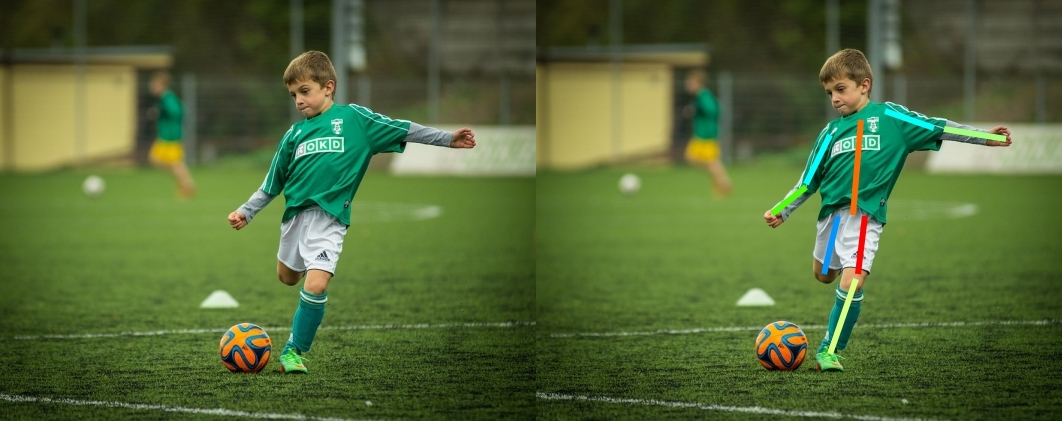
\includegraphics[width=350pt]{Imagenes/pose1.jpg}
	\centering
	\caption{Ejemplo de representación de una pose en un niño donde  se dibujan las líneas sobre los elementos más importantes que la conforman. Fuente: \url{pixabay.com}}
	\label{fig:pose1}
\end{figure}

En la figura \ref{fig:pose1}, se muestra a un niño jugando al fútbol. La pose establecida por el cuerpo del niño sugiere una acción en concreto. \par

\subsection{Poses compatibles con amenazas y agresiones}

La configuración de la disposición de las extremidades, y su relación con el tronco del cuerpo humano, puede definir qué pose forma, y en la mayoría de los casos, la acción que se está ejecutando. \par

Si bien, determinadas poses pueden sugerir que el sujeto observado pueda estar realizando múltiples acciones, existen determinadas poses que son mayormente compatibles para acciones concretas, como por ejemplo, las amenazas y agresiones humanas.\par

Por amenazas y agresiones humanas, se entiende como la utilización de extremidades del cuerpo para proferir amenazas y agresiones físicas a cualquier objeto presente en su entorno, o la disposición de las extremidades de manera que el sujeto pueda estar utilizando un arma para efectuar una agresión o amenaza. \par 

Es posible que la agresión no sea efectuada hacia otra persona, o no se pueda visualizar qué o quién recibe la agresión, sin embargo se puede agredir a un objeto que pueda contener a un ser vivo dentro del mismo, ejemplo: una persona puede estar golpeando un auto que en su interior contiene un niño no visible para el observador.\par

A través de la observación de agresiones en imágenes con armas de fuego en Internet, se pueden citar algunos ejemplos de poses que pueden ser consideradas compatibles con agresión:

\begin{enumerate}
	\baselineskip 16pt
	\item Brazos levantados formando ángulos de entre 50 y 120 grados con el tronco (ej. una persona apuntando un arma de fuego). 
	\item Brazos levantados formando ángulos superiores a los 170 grados con el tronco (ej. una persona propinando golpes con los brazos ) 
	\item Piernas levantadas formando ángulos de entre 250 y 80 grados con el tronco  (ej. una persona propinando golpes con las piernas ) 
	\item Pueden ocurrir combinaciones de las anteriores.
\end{enumerate}

\subsection{Métodos de representación de poses}
Según Doménech (2018) existen por lo menos tres categorías de métodos de representación de poses humanas de acuerdo a como se interpreta la estructura del cuerpo:

\begin{enumerate}
	\baselineskip 16pt
	\item Métodos con enfoque generativo: utilizan un modelo del cuerpo conocido con anticipación, y lo representan a través del conjunto de sus partes unidas por restricciones impuestas a las articulaciones en la estructura del esqueleto.\par
	\item Métodos con enfoque discriminativo: en ellos no se conoce con anticipación el modelo del cuerpo sino que se utilizan algoritmos que 'aprenden' a mapear la relación entre las imágenes y las poses. Se utiliza aprendizaje supervisado o también se puede buscar poses por similitud a partir de cierto número de candidatos.\par
	\item Métodos híbridos: combinan los métodos generativos y discriminativos. \par
\end{enumerate}

Y existen también modelos para la representación de poses, siendo uno de los más utilizados el denominado \textit{Pictorial Structures Model}, PSM por sus siglas en inglés, que grafica el cuerpo a través de partes cilíndricas unidas por puntos articulares que conforman el esqueleto del cuerpo. \par
 
Estos cilindros representan partes de las extremidades, y los puntos son las articulaciones que los unen. En ellos se configuran una serie de restricciones de tamaño, movimiento y jerarquía.

\begin{figure}[h!]
	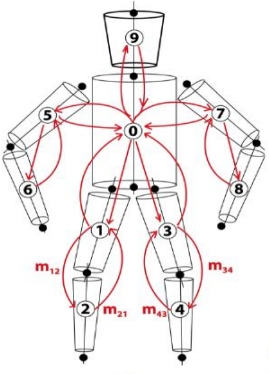
\includegraphics[width=150pt]{Imagenes/domenech1.jpg}
	\centering
	\caption{Pictorial Structures Model. Fuente: Doménech (2018).}
	\label{fig:domenech2}
\end{figure}

\newpage	
\section{Conceptos de Machine Learning}\label{machinelearning}

Se conoce como \textit{Machine Learning} (ML) en inglés, a la ciencia relacionada con Inteligencia Artificial en la cual se pueden configurar modelos matemáticos y probabilísticos para responder a situaciones de la vida real. Básicamente, se trata de entrenar algoritmos para ofrecer respuestas, bajo ciertas condiciones de campo. Su traducción literal se refiere al proceso de 'enseñar' a una máquina a responder a situaciones de manera inteligente, sin el uso de condicionales.\par
	
\subsection{Aprendizaje y entrenamiento}
El aprendizaje se da solamente en ciertos seres vivos del planeta, por lo que el concepto era ajeno a las máquinas, hasta ahora: consiste en incorporar conocimientos de situaciones repetitivas para poder responder con una acción o simplemente establecer un registro del mismo. En el ámbito de la computación, se adoptó el concepto de aprendizaje y entrenamiento al proceso de preparar y parametrizar, con datos de entrada, un modelo matemático o algoritmo para que pueda responder, con datos de salida, de la misma manera que lo haría un ser vivo.\par

Para entender el concepto, considérese a los datos de entrada como estímulos para el aprendizaje, donde ciertos pesos (parámetros) influyen en la importancia de cada uno, y donde se genera un valor de salida aprendido.\par

En el entrenamiento de un modelo matemático, se parametriza el mismo con estos estímulos y los pesos para cada estímulo, ajustando los mismos a modo de que el resultado se aproxime a un valor esperado.  \par

Existen numerosos métodos que utilizan funciones para aproximar estos resultados (función costo, descenso de gradiente, etc), pero no se profundizará sobre los mismos. \par

A partir de este punto, se hace referencia a los datos de entrada para el proceso de aprendizaje, como Input Dataset -o Features-, y la obtención de resultados de salida -o simplemente Output-.\par

\subsubsection{Aprendizaje supervisado}

Aprendizaje supervisado es el proceso de entrenar un algoritmo con datos de entrada estructurados, y en donde se conoce o se espera algún tipo de dato de salida previamente conocido (Marsland, 2014) .\par

En el aprendizaje supervisado, se conoce acerca de la naturaleza de los datos de entrada, y se esperan datos de salida del mismo modo. Por ejemplo, se puede estimar el costo de una casa a partir de ciertos datos conocidos, como el área, cantidad de pisos, ubicación, etc.  \par

Entonces se tienen datos precisos, catalogados sobre características de la casa, y además se espera un valor costo, o sea, se conoce la naturaleza del resultado.\par

\subsubsection{Aprendizaje no supervisado}

Por el otro lado en el aprendizaje no supervisado, no se conoce la clasificación de los datos de entrada ni de salida. Los datos de entrada no poseen una estructura definida, no están catalogados y no se sabe acerca de los datos de salida esperados (Marsland, 2014). Algunos ejemplos de datos de entrada para el aprendizaje no supervisado podrían ser: datos de audio, imágenes o texto. En este tipo de aprendizaje priman los problemas de clasificación de patrones como el de textos extensos de acuerdo a una característica en particular.\par

\section{Métodos de clasificación}\label{clasificacion}
A continuación, un breve resumen acerca de algunos modelos probabilísticos utilizados en Machine Learning, para clasificar datos. No se profundizarán conceptos sobre todos los modelos, solamente aquellos que sirvieron para la realización de este trabajo. \par

Bailey et al. (2007) describe algunos métodos principales de clasificadores, también se puede agregar los citados por Kamarudin et al. (2015), y los métodos de regresión de Andrew Ng en su curso de Machine Learning. \par

\subsection{Regresión Lineal}

La regresión lineal es un modelo matemático utilizado para aproximar la dependencia de dos variables, se utiliza como clasificador binario: solo devuelve dos posibles datos de salida. Este tipo de clasificador se utiliza para determinar si un objeto es o no es de cierto tipo. \par
Representación de hipótesis: \textit{h(x) = b + $b_1$$x_1$ + $b_1$$x_1$....+ $b_n$$x_n$}
	
Donde \textit{b} son los pesos de cada entrada, también llamados parámetros (se utilizan para modificar la importancia de cada variable), \textit{x} son los features, e \textit{y} es el resultado devuelto/esperado. Fíjese que la función hipótesis tiene la forma de una ecuación de recta, de ahí su nombre. \par


Si se dibujaran los datos de salida del clasificador en un plano cartesiano, se podrían separar los valores por medio de una línea recta -denominada límite de decisión-. \par

Una unidad de datos de entrenamiento puede identificarse como \textit{(x, y)} donde \textit{x} representa los datos de entrada, e \textit{y} representa el de salida esperado. Además, para la regresión lineal, se puede utilizar una variable de entrada, o múltiples variables de entrada, siendo \textit{m} la cantidad de variables de entradas -cantidad de features- y \textit{n} la cantidad de conjuntos de entrenamiento.  \par

\begin{figure}[h!]
	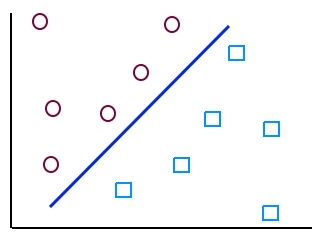
\includegraphics[width=180pt]{Imagenes/regresion1.jpg}
	\centering
	\caption{Regresión lineal, datos de salida en un plano cartesiano con el límite de decisión. Fuente: Andrew Ng, Machine Learning Course, www.coursera.org.}
	\label{fig:regresion1}
\end{figure}


\subsection{Regresión Logística}

La regresión logística también se utiliza como clasificador binario, pero se diferencia de la Regresión Lineal en que los datos de salida, en el plano cartesiano, están separados por una línea curva, o circular: esto es porque el límite de decisión esta representado por una ecuación cuadrática. La representación de su hipótesis utiliza la función denominada función logística o sigmoidea. \par

También, como la regresión lineal, la logística puede utilizar una o varias variables de entrada denotadas por la letra \textit{x}, y la salida por la letra \textit{y}, además de \textit{m} y \textit{n} que continúan teniendo el mismo significado. \par

Representación de hipótesis: \textit{h(x) = g($O^t$x)}
donde \textit{z = $O^t$x}
entonces 
\begin{equation}
	g(z) = \frac{1}{1 + e\raisebox{1ex}{-z}} 
\end{equation}

Donde \textit{z} es la función cuadrática con los valores de los datos de entradas. \par

Ejemplo: \textit{z = O + $O_1$$x^2_1$ + $O_2$$x^2_2$}  es la ecuación de la circunferencia, que puede ser utilizado como límite de decisión.

\begin{figure}[h!]
	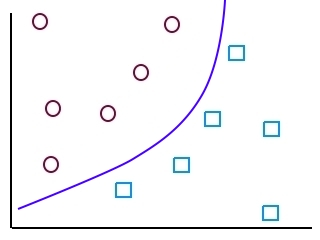
\includegraphics[width=180pt]{Imagenes/regresion2.jpg}
	\centering
	\caption{Regresión logística, datos de salida en un plano cartesiano con el límite de decisión. Fuente: Andrew Ng, Machine Learning Course, www.coursera.org.}
	\label{fig:regresion2}
\end{figure}

\subsection{Máquinas de Vectores Soporte}

En inglés \textit{Support Vector Machines} (SVM) es un método de clasificación que utiliza funciones matemáticas: dado un conjunto de puntos donde cada uno pertenece a una de dos posibles categorías, se construye un modelo capaz de predecir si un punto nuevo pertenece a una de las dos categorías.  \par

Pertenece a la categoría de los clasificadores lineales, puesto que inducen separadores lineales o hiperplanos. \par

Básicamente, se busca una linea que separe los puntos de entrenamiento en dos áreas diferentes en un gráfico. El algoritmo SVM halla la ecuación de recta óptima.\par

Mediante una función, se intenta determinar si un dato de entrada (nuevo punto en el gráfico) pertenece o no a uno de los dos grupos establecidos mediante la separación realizada. \par

Así, la separación de datos en el plano cartesiano se efectúa mediante un hiperplano, buscando aquel que sea óptimo: esto es, el hiperplano cuya distancia sea igual a los puntos más cercanos a la recta.\par

\begin{figure}[h!]
	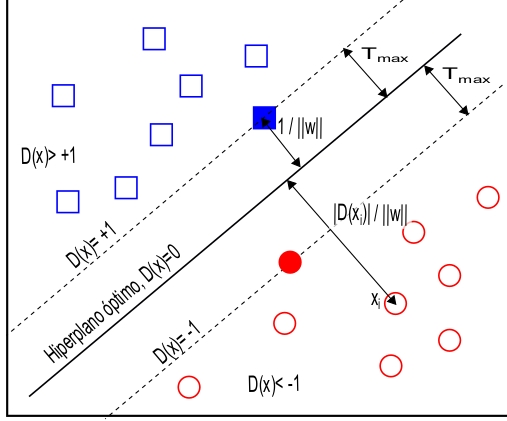
\includegraphics[width=200pt]{Imagenes/svm1.jpg}
	\centering
	\caption{SVM con hiperplano óptimo. Fuente: Suarez (2014) }
	\label{fig:svm1}
\end{figure}

\subsubsection{SVM Multiclase}
Un clasificador lineal solo puede diferenciar una clase de objeto, del resto de objetos. La separación por medio de una función lineal muchas veces no es aplicable a ciertos problemas, o las clases no son perfectamente separables. \par

Esto se soluciona con funciones kernel, que proyectan la información del universo de datos a una dimensión extra. Para darnos una idea, se podría pensar primero en el conjunto de datos en un plano cartesiano, que, como se sabe, es un gráfico de dos dimensiones (x e y) con líneas abscisas y una línea recta divide los puntos que representan los datos. La función kernel permite agregar una dimensión extra, como un cubo de tres dimensiones donde ciertos datos tendrían valores en otra dimensión, como si el plano tuviese profundidad. \par

Algunos tipos de funciones kernel son (Suarez 2014): 
\begin{enumerate}[noitemsep]
	\item Polinomial.
	\item Perceptrón.
	\item Gaussiana.
	\item Sigmoidea.
\end{enumerate}

Con las funciones kernel, se podría por ejemplo, mapear los valores de ciertos puntos, que bajo un plano de dos dimensiones no son perfectamente separables mediante una linea recta, haciendo de ese modo que los nuevos puntos sean separables.

\subsection{Redes Neuronales Artificiales}

En biología, una neurona es un tipo de célula del sistema nervioso que es capaz de comunicar pulsos eléctricos a otras células. El cerebro humano esta compuesto por miles de millones de estas células, y en la combinación de estas es donde se producen los procesos neuronales que permiten controlar partes del cuerpo, aprender y sentir. \par

La estructura básica de una neurona consiste en (Matich, 2001):
\begin{compactitem}
	\item Dendritas: conexiones que permiten la comunicación de otras neuronas con la actual.
	\item Núcleo: donde se realiza el proceso celular.
	\item Axón: comunica la señal generada por el núcleo a otra neurona en la red.
\end{compactitem}

\begin{figure}[h!]
	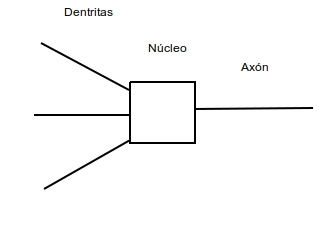
\includegraphics[width=220pt]{Imagenes/neurona.jpg}
	\centering
	\caption{Estructura superficial de una neurona natural. Fuente: Matich (2001).}
	\label{fig:haarlike1}
\end{figure}

Las redes neuronales artificiales simulan la interconexión de las neuronas cerebrales. Se asignan un conjunto de variables de entrada a diferentes resultados de salida a través de nodos intermedios por los cuales van circulando los datos. Los nodos intermedios pueden ser muchos, o simplemente pueden no existir, dependiendo de las necesidades del modelo. \par

\subsection{Arquitectura de una red neuronal artificial}
Ahora que se conoce el concepto básico de una neurona, se podría imaginar el tener varias neuronas interconectadas entre sí, donde, teniendo datos de entrada (estímulos), estos de propagan a través de la estructura hasta llegar al final, devolviendo un valor de salida\par

Entre cada conexión de neuronas existe un parámetro denominado \textit{peso} de la conexión, que es nada mas que un parámetro modificable y adaptable al proceso de aprendizaje. La modificación de los pesos, es lo que se denomina aprendizaje, y existen diferentes métodos de modificar los pesos a medida que se va iterando la red.\par

\begin{figure}[h!]
	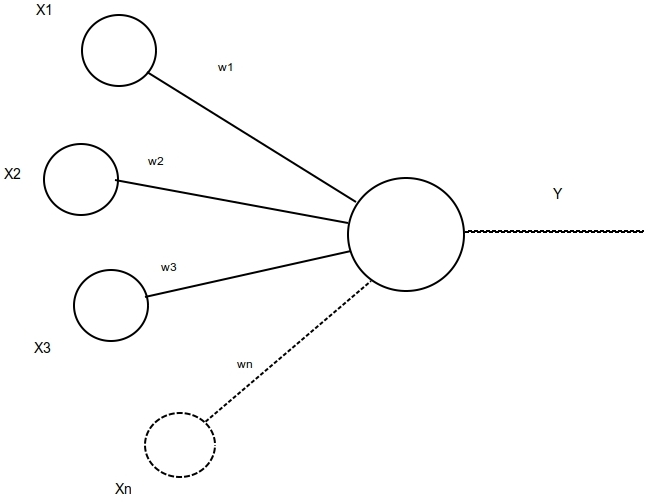
\includegraphics[width=340pt]{Imagenes/network1.jpg}
	\centering
	\caption{Estructura de una red neuronal simple. Fuente: Matich (2001).}
	\label{fig:network1}
\end{figure}

En la figura \ref{fig:network1}, se puede observar una estructura neuronal simple, de una capa de neuronas de entrada, y otra capa de una sola neurona de salida, donde \textbf{X} son las entradas para las neuronas (los estímulos), \textbf{w} son los pesos (parámetros adaptables) que existen entre las neuronas de entrada y la neurona de salida e \textbf{Y} es el resultado del proceso. \par

\subsection{Redes neuronales multicapas}

Otros modelos de redes neuronales pueden agregar más capas de neuronas entre la capa de entrada y la de salida, las cuales son denominadas \textit{capas ocultas}. Una red neuronal con varias capas ocultas se denomina multicapa. En la figura \ref{fig:network1}, no existen capas intermedias ocultas.

\begin{figure}[h!]
	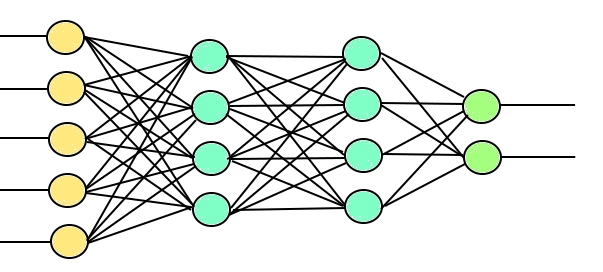
\includegraphics[width=380pt]{Imagenes/network2.jpg}
	\centering
	\caption{Estructura de una red neuronal con múltiples capas. Fuente: Matich (2001).}
	\label{fig:network2}
\end{figure}

En la figura \ref{fig:network2}, se puede observar una estructura de red neuronal con dos capas ocultas (intermedias). La capa de entrada (color naranja), con cinco neuronas, las dos capas ocultas (color celeste) con cuatro neuronas cada una, y la capa de salida (color verde) con dos neuronas.\par

\subsubsection{Perceptrón}
Es un modelo de red neuronal que permite diferenciar solo tipos de clases de forma lineal. Fué uno de los primeros modelos de redes artificiales ideados. Originalmente el perceptrón fue creado para resolver problemas de visión por computadoras, tratando de imitar cómo el cerebro aprende patrones a partir de las imágenes captadas por los ojos.\par

El problema del perceptrón, es que solamente podía clasificar patrones linealmente separables, y no era posible ajustar los pesos de todas las capas, ya que no se diseñó un algoritmo para tal fin.\par

Con el correr de los años, el perceptrón quedó olvidado ya que sus limitaciones lo hacían inservible para problemas más complejos. Durante más de dos décadas, no hubieron avances sobre redes neuronales hasta la llegada del algoritmo de \textit{backpropagation}.\par

\subsubsection{Backpropagation}
Del inglés \textit{back propagation}, o propagación hacia atrás, es un algoritmo de aprendizaje supervisado (para el ajuste de pesos) que, dado un valor de salida de la red neuronal, calcula la diferencia con respecto a la salida deseada y ajusta los pesos de las conexiones de las capas de adelante hacia atrás.\par

El algoritmo de backpropagation empieza cuando ha terminado la propagación hacia adelante, es decir, cuando se ha conseguido valores en la capa de salida. Una vez obtenidos los valores, se comparan los mismos con los valores de salida deseados -ésto se denomina \textit{cálculo de error}-, y un algoritmo recursivo va ajustando los pesos en las capas anteriores hasta llegar a la capa de entrada donde termina el backpropagation.\par

No se profundizará sobre el algoritmo matemático del backpropagation ya que no es la finalidad de este trabajo explicar detalladamente estos conceptos, solo dar una breve descripción de su funcionamiento.\par


\subsubsection{Tasa de aprendizaje}
En inglés \textit{learning rate}, es un parámetro de redes neuronales que determina la cantidad de ciclos de entrenamiento en la que la red actualizará sus pesos, así, a menor tasa los parámetros se actualizarán una mayor cantidad de veces y a tasa superior, la red actualizará sus pesos con menor frecuencia.

\subsubsection{Función de pérdida}
\textit{Loss function} en inglés, es una parte importante de las redes neuronales artificiales que mide la inconsistencia entre valores predichos y el valor de salida esperado. \par

De esta manera, la función de pérdida retorna un valor numérico que determina la robustez de la red neuronal. A un valor menor de la pérdida, mayor es la precisión obtenida.\par

\subsubsection{Optimizadores de redes neuronales artificiales}
Los optimizadores son algoritmos utilizados para minimizar la función objetivo, que es básicamente una función matemática dependiente de los parámetros de aprendizaje del modelo de la red neuronal. No se profundizará sobre el funcionamiento de los optimizadores. \par

Algunos de los optimizadores más conocidos son:
\begin{itemize}
	\item Descenso de gradiente: utilizado para ajustar los pesos en los ciclos de entrenamiento.
	\item Adam: calcula la tasa de aprendizaje de una red manteniendo un promedio de gradientes de ciclos anteriores.
	\item Adagrad: simplemente la tasa de aprendizaje de una red de acuerdo a los parámetros de la misma.
\end{itemize}

\subsection{Funciones de capas de redes neuronales artificiales}

\subsubsection{Funciones de entrada}
Hasta ahora se ha enfocado en la estructura de una red neuronal y el modo en que se ajustan los pesos de acuerdo a una salida pero no se ha mencionado el modo en que se obtiene la misma.\par

Cada capa de la red neuronal está compuesta por neuronas interconectadas con las capas adyacentes, pero además, cada neurona de cada capa implementa una función de acuerdo al tipo de capa (entrada, oculta o salida). Esta función es la encargada de procesar el valor de entrada y devolver un valor de salida, o estado de la neurona.\par

La capa de entrada implementa lo que se denominan funciones de entrada, y solamente existen ciertas funciones que pueden aplicarse a las neuronas de la capa de entrada.\\ \par 

De Matich (2001) se pueden entresacar los tipos de funciones de entrada más comunes:
\begin{enumerate}
	\item Sumatoria de entradas pesadas: suma de todos los valores de
	entrada de la neurona, multiplicados por sus correspondientes pesos.\par 
	
	\[\sum \textit{($n_i$$W_i$)} \]
	
	\item Productoria de entradas pesadas: producto de todos los valores de entrada de la neurona, multiplicados por sus correspondientes pesos.\par 
	
	\[\prod \textit{($n_i$$W_i$)} \]

	\item Máximo de las entradas pesadas: toma el producto más alto de la multiplicación de valores y sus pesos correspondientes.\par 
	
	\[ \textit{Max($n_i$$W_i$)} \]
	
\end{enumerate}


\subsubsection{Funciones de activación}
Ahora, una capa oculta también puede tener una o más neuronas interconectadas con las capas adyacentes: la neurona recibe datos de la capa anterior, procesa los datos, y envía su estado a la siguiente capa.\par

Así como las funciones de entrada, las funciones de activación solamente son aplicables a las capas intermedias ocultas, aunque existen solo un par de funciones aplicables a más de una capa.\par

En biología, una neurona puede estar activa o inactiva, en las redes artificiales sucede lo mismo: una neurona puede estar activa o inactiva de acuerdo al valor devuelto por la función de activación de la misma.\par

Una función de activación recibe datos de entrada y genera un resultado de activación. Generalmente pueden tomar valores de 0 y 1, o -1 y 1 (desactivado y activado). Existen funciones que pueden devolver más estados.\par

De Enyinna et al. (2018) se pueden citar tres de los tipos de funciones de activación más conocidos:

\begin{enumerate}
	\item Función sigmoidea: es una función de activación no lineal, conocido también como función logística. Su uso mayor se da en redes neuronales aunque se ha comprobado que tiene ciertos problemas con backpropagation, y otras funciones más modernas se utilizan en su lugar. Esta función tiene algunas variantes que no se detallarán en este trabajo. Su ecuación es:\par 
	
	\begin{equation}
	f(x) = \frac{1}{1 + e\raisebox{1ex}{-x}} 
	\end{equation}

	\item Función tangente hiperbólica: es una función de activación utilizada muchas veces en lugar de la función sigmoidea ya que ofrece mejores velocidades de entrenamiento en redes neuronales multicapa. Su ecuación:\par 

	\begin{equation}
	f(x) = \frac{e\raisebox{1ex}{x} - e\raisebox{1ex}{-x}}{e\raisebox{1ex}{x} + e\raisebox{1ex}{-x}} 
	\end{equation}

	\item ReLU: \textit{Rectified linear unit}, viene del inglés, o Unidad linear rectificada es una función de activación más moderna y que se ha comprobado ofrece velocidades de entrenamiento muy superiores a las anteriores. \par 
	Representa algo parecido a una función linear por lo que resulta rápido para procesos de entrenamiento intensivos. Actualmente es la función de activación más utilizada ya que ha demostrado una eficiencia de velocidad y generalización (aplicable a múltiples modelos) bastante altos.	ReLU aplica un umbral simple a los valores de entrada separando los mismos de acuerdo a una regla establecida por su ecuación:\par 

	\[ \textit{f(x) = Max(0, x)} \]
	
	donde:
	
	\[ \textit{x, si x $ >= $ 0} \]
	\[ \textit{0, si x $ < $ 0} \]

	ReLU además cuenta con otras variantes que aplican distintos tipos de umbrales pero no se detallarán en el presente trabajo.\par 
\end{enumerate}	

\subsubsection{Funciones de salida}
La capa de salida también implementa ciertas funciones, citando:\par

\begin{enumerate}[noitemsep]
	\item Función lineal: También llamada función identidad. 
	\item Función sigmoidea: ya detallada anteriormente. 
\end{enumerate}

\section{Visión por computadora}\label{visionporcomputadora}

En los últimos años, los problemas de visión por computadora, junto con con los de reconocimiento de actividad humana, han acaparado los trabajos e investigaciones en inteligencia artificial, dada la cantidad de situaciones en las cuales es necesario utilizar ayuda no humana para resolver problemas. Los sistemas computacionales han evolucionado y la inteligencia artificial ha surgido como una ciencia de estudio capaz de proveer la ayuda necesaria. \par

La representación de una imagen, en términos informáticos, es la agrupación de números distribuidos en una matriz, los cuales simbolizan intensidades de color y luminosidad. Sin embargo, un conjunto de componentes electrónicos no es capaz de entender una imagen.\par

\subsection{Detección y reconocimiento de objetos en imágenes}

Los sistemas de vigilancia en auge actualmente son los de segunda generación que son los dispositivos que capturan imágenes para ser  enviadas a procesadores obteniendo la información relevante de las mismas a través de algoritmos computacionales. \par

Si bien existen investigaciones enfocadas a la utilización de Inteligencia Artificial para la Vigilancia Inteligente, resulta por ahora una tarea difícil de implementar debido a la cantidad de combinaciones posibles de escenarios que puedan darse, la cantidad de datos de entrada y los patrones que se deben analizar en las diferentes fases. \\ \par

Normalmente, el proceso de identificación de objetos en imágenes se da en diferentes etapas descritas por Lozano (2010) y Kamarudin et al. (2015), ellas son:	
\begin{enumerate}[label=\alph*)]
	\item \textbf{Detección de objetos.}\\
		La detección de objetos en imágenes es una de las áreas de mayor investigación en visión por computadora. La tarea no resulta fácil, ya que existen numerosos elementos a tener en cuenta para la detección de objetos que sean de relevancia. \par
		
		El principal obstáculo, es determinar si un conjunto de pixeles forman o no un objeto tomando en cuenta que existen innumerables combinaciones de posición, luminosidad, color y formas, como así también el ruido de interferencia y el tamaño del objeto (o su lejanía de la cámara).\par
		
		Enfocado a la seguridad, la detección de objetos trata de identificar solamente unas pocas categorías de objetos en imágenes, lo que lo hace un proceso más viable: la detección de formas humanas, también denominado detección de peatones (Pedestrian detection en inglés).
		
		\textbf{Técnicas de detección de objetos en imágenes}\\
		A través de los años, como consecuencia de las investigaciones en visión por computadora, han surgido diferentes enfoques en la utilización de técnicas de detección de objetos, Valera y Velastin (2005) citan dos enfoques a lo que se pueden agregar además el presentado por Nidhi (2005) y Barron et al. (2015):
		\begin{itemize}
			\setlength\itemsep{-1.2em}
			\item Diferencia temporal: 
			este enfoque se basa en la comparación de un frame (imagen de video) con el frame anterior. Esta acción permite identificar objetos en movimiento cambiante dentro del conjunto de frames, aunque sugieren que es un proceso más lento que otros.\\	
			\item Substracción de fondo: utiliza una imagen de fondo que se compara con frames pixel a pixel para determinar los cambios ocurridos en la imagen, lo que permite obtener contornos de objetos.\\
			\item Filtrado: este método es quizás el menos utilizado ya que las características de los objetos suelen ser variantes. Este método sugiere la detección de objetos basados en el filtrado de color del mismo: se extraen los pixeles que concuerdan con el color de un objeto previamente establecido. Como los objetos pueden variar su color, o luminosidad, este método resulta poco efectivo. Puede utilizarse en condiciones muy controladas.\\
			\item Flujo óptico: este método es el más costoso computacionalmente hablando, ya que determina vectores de movimiento de cada uno de los pixeles para determinar el contorno de un objeto en movimiento dentro de un frame. Cada pixel en movimiento (posición inicial y posición final) determina un vector, un sentido de movimiento. Se puede tomar el conjunto de vectores de todos los pixeles para determinar la existencia de un objeto en la imagen.\\
		\end{itemize}
	\item \textbf{Clasificación (identificación) de objetos.}\\
		La última etapa, luego de la detección de objetos, es la clasificación de los mismos: se debe determinar la clase de objeto detectado. Es de vital importancia poder identificar el tipo de objeto detectado, especialmente cuando se trata de personas: se necesita registrar y catalogar el comportamiento de objetos de tipo persona para determinar si se produce una forma compatible de agresión.\par
		
		\textbf{Técnicas de clasificación}\\
		Para determinar la clase de objeto extraído de una imágen, se utilizan dos tipos principales de técnicas citadas por Lozano (2010):
		\begin{itemize}
			\setlength\itemsep{-1.2em}
			\item Clasificación basada en formas: es la técnica más sencilla y consiste en, una vez identificado un objeto en una imágen, compararlo con formas de objetos existentes. Se asocia un valor numérico para identificar el grado de similitud entre las imágenes comparadas. El valor más alto asociado definirá la clase de objeto.\\
			\item Clasificación basada en movimiento: estudia el movimiento hecho por un objeto en particular, con respecto a su forma o silueta. Se sabe por ejemplo, que el cuerpo humano va cambiando su forma -esto es, existe movimiento- a través de las imágenes. 
		\end{itemize}
		
		\textbf{Métodos de clasificación}\\
		Ya se han citado las técnicas que mayormente se utilizan en la clasificación de objetos, además de que existen otras técnicas menos conocidas o que producen resultados menos certeros, ahora hay que hablar sobre los métodos de clasificación utilizados actualmente por programas computacionales para separar objetos según su clase utilizando las técnicas citadas previamente.\par
		
		Aunque algunos de ellos ya fueron citados y explicados en otros capítulos de este trabajo, ahora solo se citarán aquellos que fueron implementados en la clasificación de objetos en imágenes como ser: Árboles de decisiones, Support Vector Machines, Redes bayesianas y Redes Neuronales Artificiales.\par
	\item \textbf{Extracción de características (features) de objetos.}\\
		Características de objetos pueden ser su contorno, medidas, color o disposición. Las técnicas de extracción se basan en el procesamiento digital de imágenes mediante herramientas que permiten aplicar algoritmos matemáticos para determinar ciertas cualidades.\par
		Un objeto se diferencia de otro justamente por las propiedades gráficas que lo representan, y cuyos cambios determinarán su comportamiento.\par
	\item \textbf{Análisis del comportamiento de los objetos.}\\
		En esta etapa se lleva a cabo el análisis de los cambios de propiedades de un objeto, como por ejemplo su ubicación y forma establecida por el contorno. Analizar el comportamiento conlleva al seguimiento minucioso de sus propiedades.\par
		Una de las técnicas de análisis de comportamiento de objetos mas utilizada es la denominada en inglés \textit{Dynamic Time Warping} (DTW), técnica ampliamente utilizada en procesamiento de audio, que consiste básicamente en segmentar una secuencia de datos en unidades de tiempo iguales para así poder compararlas y establecer el cambio producido entre segmentos.\par 
\end{enumerate}

\subsection{Histograma de Gradientes Orientados}
En inglés \textit{Histograms of Oriented Gradients} (HOG), es una técnica de detección de objetos en imágenes, más precisamente para la detección de humanos, según Dalal y Trigg (2005). Básicamente, se trata de un descriptor de objetos, que permite caracterizarlos en un mapa de gradientes. Se suele utilizar HOG como descriptor de objetos y SVM como clasificador para una gran cantidad de herramientas de detección y clasificación.\par

La idea básica del HOG, es dividir una imagen en ventanas (denominadas blocks, o \textit{detection windows} en inglés), obteniendo los gradientes que se forman dentro de cada ventana, así, una imagen puede contener decenas de pequeñas ventanas con sus gradientes. El gradiente contiene el vector dirección, lo que permite caracterizar la zona dentro de la ventana.\par

Un gradiente es básicamente, un vector que indica la dirección donde ocurre el cambio de luminosidad de oscuro a claro. Para un gradiente dentro de una ventana, se obtiene la representación a través de una línea que indica la separación de luminosidad ocurrida dentro de la ventana, y la dirección en la que ocurre el cambio. De esta manera, con el conjunto total de gradientes de la figura, se logra obtener una representación aproximada del contorno del objeto.\par

Además, una ventana puede contener diferentes cantidades de gradientes, de acuerdo a la cantidad de líneas tangentes a un punto. Sin embargo, las herramientas de extracción de HOGs tienen parámetros para la configuración de la cantidad de gradientes que se desean obtener, como también el tamaño de las ventanas a procesar (generalmente en pixeles). Cuanto más gradientes, más generalizado es el caso, y por el contrario, cuanto menos gradientes se obtengan, más especializado será.\par

\begin{figure}[h!]
	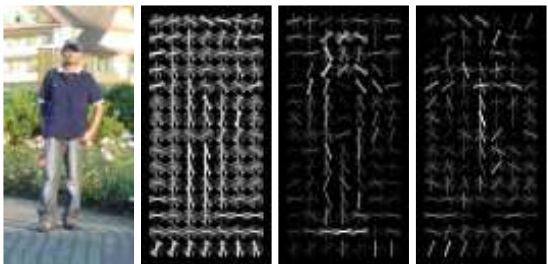
\includegraphics[width=340pt]{Imagenes/hog1.jpg}
	\centering
	\caption{imagen de un hombre, y los gradientes obtenidos de la misma. Fuente Dalal y Trigg (2005).}
	\label{fig:hog1}
\end{figure}
 

\section{Herramientas de visión por computadora}\label{herramientasdevisionporcomputadora}

\subsection{OpenCV}

OpenCV (Open Computer Vision, en inglés) es una librería escrita con participación de investigadores de Intel Corp. para el procesamiento de imágenes por computadora según lo descrito en la referencia oficial. \par 

Provee una serie de procedimientos y funciones estándar para la manipulación de imágenes en, hasta la fecha de este trabajo, tres lenguajes de programación de computadoras: C++,  Python y Java. Provee herramientas preestablecidas y preconfiguradas para que la tarea del programador sea más fácil y rápida. \par

OpenCV se escribió con la finalidad de ser eficiente y aprovechar las instrucciones de bajo nivel de los procesadores Intel, que tienen una cuota muy alta de ventas en el mercado mundial. Esto, sumado a que fue escrito en C y C++, hace que el código se ejecute mucho más rápido que otras librerias de procesamiento de imágenes.\par

Además, la librería ofrece bibliotecas de funciones y procedimientos parametrizables para resolver problemas de Inteligencia Artificial. Los componentes prefabricados con un alto nivel de abstracción hacen posible al programador implementar, por ejemplo, un clasificador de objetos en unas pocas líneas de instrucciones Python. Los módulos de inteligencia artificial mas conocidos de OpenCV son:\par
\begin{itemize}
	\setlength\itemsep{-0.2em}
	\item Clasificadores en cascada	
	\item Clasificadores Bayes
	\item Support Vector Machines
	\item Decision Trees 
	\item Redes neuronales 
\end{itemize}

En este trabajo, no se detallarán sobre los módulos de tratamiento de imágenes de OpenCV, ya que no se utilizaron durante el desarrollo. En su lugar, se abordarán conceptos y detalles sobre algunas de las librerías OpenCV de Inteligencia Artificial que fueron utilizadas.\par

\subsubsection{Clasificadores en Cascada}

Llamados en inglés \textit{Cascade of Boosted Classifiers working with Haar-like Features}, es un módulo OpenCV que implementa una serie de clasificadores que son utilizados para detección de objetos en imágenes. Éstos están dispuestos en una estructura de cascada de manera que puedan funcionar más rápidamente que un clasificador único y pesado. La salida de unos clasificadores pasan a ser las entradas de otros, formando así como una especie de puertas lógicas donde se cumplen condiciones, para tener un resultado final. \par

La palabra \textit{boosted} además, hace referencia a que estos clasificadores implementan técnicas de Machine Learning que aceleran el entrenamiento de manera eficiente, actualmente se implementan cuatro técnicas conocidas como: \textit{Discrete Adaboost, Real Adaboost, Gentle Adaboost y Logitboost}. No se detallarán sobre estas técnicas en el presente documento.\par

Las entradas de datos para estos clasificadores, se conocen en inglés como \textit{Haar-like features}. Cada clasificador simple que compone la cascada recibe solo un tipo de entrada (feature), que en combinación con los demás clasificadores, pueden determinar la clase de objeto en proceso. La entrada es un conjunto de pixeles con una distribución en particular, como se detalla en la figura \ref{fig:haarlike1}.\par

\begin{figure}[h!]
	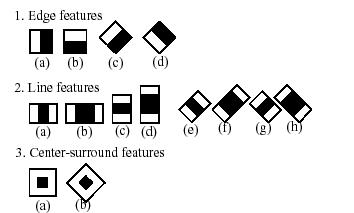
\includegraphics[width=240pt]{Imagenes/haarlike.jpg}
	\centering
	\caption{Entradas (Features) para los distintos clasificadores en cascada Fuente: OpenCV Reference Manual.}
	\label{fig:haarlike1}
\end{figure}

\subsubsection{Redes Neuronales Profundas}
En inglés \textit{Deep Neural Networks}, y se las conocen por sus siglas como DNN. Son redes neuronales multicapa donde existen niveles de capas ocultas agrupadas, y cada grupo procesa datos para generar una representación mas abstracta del objeto de proceso (Matich, 2001), de ahí el adjetivo de profundas.\par

Existen DNNs que pueden llegar a implementar 256 capas intermedias con hasta 128 entradas y el mismo número de neuronas, y es solo un ejemplo básico. Estas redes neuronales tienen modelos extremadamente enormes y requieren procesadores potentes, sin mencionar que los ciclos de entrenamiento pueden durar un par de días.\par

La ventaja de utilizar DNNs es que permite resolver problemas complejos no lineales, aunque la exactitud muchas veces depende de cuan entrenado esté el modelo.\par

En visión por computadora, se utilizan DNNs para identificar múltiples objetos, también o para extraer poses humanas en imágenes, como ejemplos.\par

\subsubsection{Redes Neuronales Convolucionales}
En inglés \textit{Convolutional Neural Networks}, CNN por sus siglas, es otro tipo de redes neuronales cuyo modelo es parecido al del perceptrón multicapa. Este tipo de redes es utilizado para la segmentación y clasificación de imágenes debido a que, por la naturaleza de su modelo, es aplicable en mayor grado a los problemas de visión por computadoras.\par

En las redes convolucionales, se aplican ciertos filtros a las imágenes mediante neuronas convolucionales resumiendo así ciertas porciones de la imagen y obteniendo una representación más general de la misma, este proceso de resumir porciones se denomina reducción de muestreo, y en inglés se lo conoce como \textit{pooling} (pooling layer, es la capa encargada de resumir porciones de la imágen). \par

La idea detrás de las redes convolucionales, según LeCun et al. (1998) es simular el comportamiento de los receptores de la corteza visual en los cerebros biológicos mediante modelos de neuronas artificiales. \par

\newpage
\chapter{Marco metodológico}
\section{Pruebas de estimación de poses humanas}\label{pruebaspose}

Dentro de los objetivos específicos de este trabajo se cita el de obtener patrones de poses humanas captadas en imágenes secuenciales.\par

La estimación de pose es, en términos simples, la extracción de datos  de los puntos que conforman ciertas partes del cuerpo humano, con los cuales se puede diagramar la ubicación de las mismos, y la dependencia entre ellas, logrando así graficar la estructura de una pose humana.\par

Otros trabajos lo denominan esqueletización u obtener el esqueleto, pero la idea es siempre la misma, obtener un mapa de la disposición de las extremidades del cuerpo humano como si se tratase del mismo esqueleto.\par

\subsection{Prueba 1: Clasificador SVM-HOG}

\subsubsection{Justificación}
Las herramientas de software actuales de extracción de poses requieren grandes prestaciones de hardware para funcionar en tiempo real y sin retrasos importantes. En la mayoría de las páginas consultadas recomiendan procesadores de 8 núcleos, tarjetas gráficas (GPU) nVidia para el proceso en paralelo mediante la tecnología CUDA de nVidia, que permite la ejecución en paralelo utilizando los procesadores gráficos de éstas tarjetas.\par

Debido a que el desarrollo y ejecución del software se realizó sobre una computadora de dos núcleos, sin tarjetas gráficas nVidia que permitan el multiprocesamiento en paralelo se optó primero por crear un extractor de pose basado en un clasificador SVM-HOG. La idea era desarrollar un extractor de poses capaz de ejecutarse en máquinas de bajo rendimiento.\par

Con la utilización de lo mencionado en capítulos anteriores referente al significado y funcionamiento de los descriptores HOG y de los clasificadores SVM, que permiten la detección de objetos en máquinas de gama media, sin la necesidad de contar con unidades de procesamiento de alto rendimiento, se busca desarrollar un detector de objetos, personalizado y entrenado con imágenes de cuerpos humanos, para luego determinar la ubicación de los miembros del cuerpo a fin de generar una pose asociada.\par

Una vez entrenado el detector de objetos, éste será capaz de identificar cuerpos humanos en imágenes y devolver información de las anotaciones enlazadas al tipo detectado. \par

Se establece que cada clase de objeto es nada más que una persona en una configuración de pose distinta a las anteriores; cada forma humana es una clase de objeto diferente, aprovechando el término multiclase. Es decir, no se detectarán diferentes tipos de objetos conceptualmente hablando, sino que solamente se detectarán humanos en situaciones distintas según su pose. \par

Los siguientes pasos fueron llevados a cabo para obtener un extractor de poses personalizado:

\begin{enumerate}
	\setlength\itemsep{-0.2em}
	\item Recolección de imágenes del cuerpo humano.
	\item Categorización de acuerdo a, si es parte superior del cuerpo (tronco, hombros y brazos), o parte inferior del cuerpo (caderas, piernas y pies).
	\item Generación de anotaciones con información de los puntos relevantes.
	\item Implementación de múltiples detectores HOG-SVM.
	\item Entrenamiento del detector para su utilización posterior.
\end{enumerate}

\subsubsection{Descripción}

\begin{itemize}
	\item Recolección de imágenes del cuerpo humano.

	Consiste en recolectar cuadros de imágenes de diferentes secuencias que describan el cuerpo humano en alguna pose determinada.\par 
	
	Para la recolección de los cuadros, se utilizaron imágenes de un video descargado de Internet en el que, justamente, se puede observar a ciertos individuos con poses compatibles con amenazas o agresiones.\par 
	
	\begin{figure}[h!]
		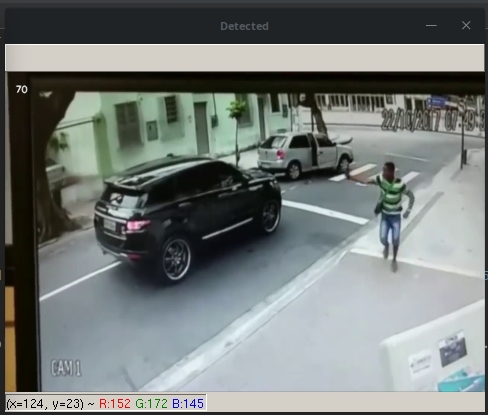
\includegraphics[width=175pt,height=130pt]{Imagenes/video1.jpg}
		\centering
		\caption{Una de las imágenes del video de pruebas donde se observa una persona posiblemente en pose de amenaza con arma de fuego corta.}
		\label{fig:video1}
	\end{figure}
	
	Para que la tarea fuera más sencilla, se escribió un programa en lenguaje Python capaz de extraer las imágenes separadas de una secuencia en vídeo.\par 
	
	Primero, se procedió a individualizar cada imagen del conjunto de imágenes del video para almacenarlas en archivos de imagen en el disco.\par 

\item{Categorización}\par

	Estas imágenes, catalogadas en el punto anterior, luego son cargadas con otra herramienta escrita en Python creada para establecer la ubicación de ciertos puntos que puedan ayudar a definir la pose. Cada punto ubicado en la imagen se guarda asociándolo con, además de sus coordenadas, una etiqueta descriptiva:
	\begin{enumerate}
		\item \textit{mi md}: manos izquierda y derecha.
		\item \textit{ci cd}: codos izquierdo y derecho.
		\item \textit{p}: pecho.
		\item \textit{c}: cadera.
		\item \textit{ri rd}: rodillas izquierda y derecha.
		\item \textit{pi pd}: manos izquierda y derecha.
	\end{enumerate}	
		
	\begin{figure}[h!]
		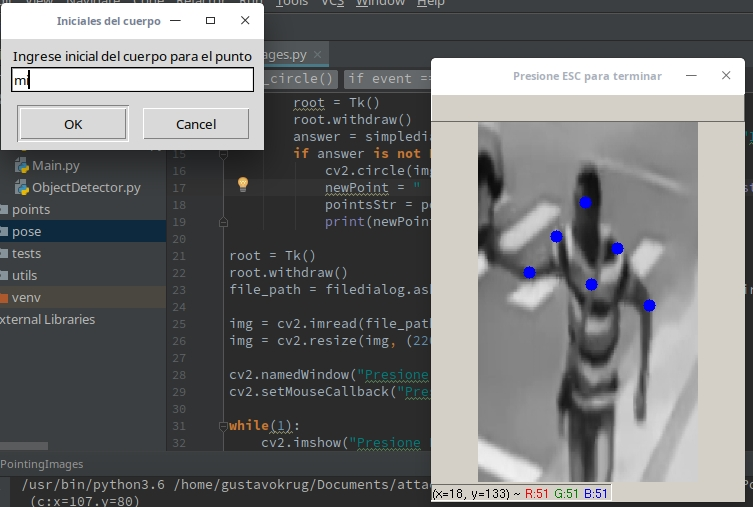
\includegraphics[width=310pt, height=150pt]{Imagenes/pose5.jpg}
		\centering
		\caption{Herramienta que permite ubicar los puntos relevantes y asociarlos a una etiqueta descriptiva.}
		\label{fig:pose5}
	\end{figure}
	
	
			
\item{Generación de anotaciones con información de los puntos relevantes}\par
	
	Una vez obtenidas las coordenadas de los puntos y la etiqueta que identifica la configuración de la disposición de estos, se procede a almacenarlos en un archivo de texto en disco.\par 
	
	Cada configuración de pose distinta, con sus imágenes y anotaciones es almacenada en un directorio diferente a fin de poder agrupar la representación de un objeto con sus anotaciones.\par 
		
		
		
\item{Implementación de múltiples detectores HOG-SVM }\par
	
	Existen numerosas librerías para Inteligencia Artificial escritas para el lenguaje Python, una de las más utilizadas es \textit{dlib}. Esta herramienta fue originalmente escrita para proveer librerías Machine Learning en C++, aunque se puede compilar para su utilización en Python. Se usa en la industria y en el ámbito de la educación para facilitar el desarrollo de software enfocado a la inteligencia artificial.\par
	
	En la documentación de la página oficial de dlib \url{http://www.dlib.net} pueden encontrarse numerosos ejemplos de casos de uso, como el que compete a este trabajo que es entrenar un detector de objetos personalizado.\par
		
	dlib provee por defecto, un detector de objetos que implementa HOG-SVM prefabricado, configurable de acuerdo a las necesidades del desarrollador. Y aunque esto facilita mucho la tarea ya que no se necesita escribir desde cero, tiene como principal limitación el hecho de que el desarrollador no puede hacer uso de un clasificador multiclase. El clasificador embebido solamente puede clasificar uno-a-muchos, es decir, puede determinar, de un conjunto de objetos, aquel objeto que coincide con los datos de entrenamiento, pero no puede determinar la clase de objetos a la cual pertenecen los demás elementos.\par
	
	Para solucionar esta limitación, se escribió código Python utilizando el detector embebido de dlib, de manera a simular un clasificador multiclase, creando diferentes instancias del objeto POO que respondan a una clase en particular. Es decir, ya que cada instancia del objeto dlib puede detectar y clasificar una sola clase de objetos, se crearon varias instancias, de acuerdo al número de tipos de poses obtenidas de las imágenes de entrenamiento.\par
	
	Así, cada elemento de pose utilizado para el entrenamiento, es considerado una clase individual para un clasificador, de manera a que si se tuvieran cinco poses distintas, se instancian cinco clasificadores de dlib.\par
	
		
\item{Entrenamiento del detector para su utilización posterior}\par
	El entrenamiento de clasificadores SVM, como ya se explicó en un capítulo anterior, consiste en introducir valores al algoritmo para establecer un límite de decisión en los datos de salida, de manera que pueda responder a un nuevo valor clasificándolo según si corresponde o no, a las características de los valores de entrenamiento. En las SVM, el límite de decisión es llamado un hiperplano.\par
	
	De esta manera, las entradas para los datos de entrenamiento serán simplemente la disposición de gradientes obtenidos mediante HOG.\par
	
	Para el entrenamiento, entonces, se utilizan las imágenes individuales de cada 'clase' de pose humana almacenadas en carpetas, con sus anotaciones. Cada instancia del clasificador dlib responde a solo una de las clases de poses almacenadas. \par
	
	\begin{figure}[h!]
		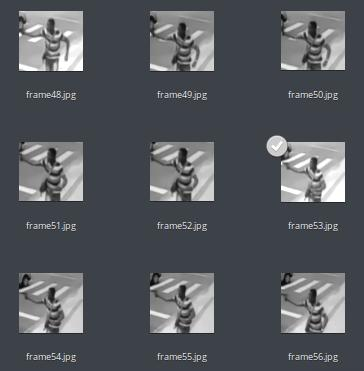
\includegraphics[width=190pt]{Imagenes/dataset1.jpg}
		\centering
		\caption{Ejemplo de secuencias de imágenes utilizadas para el entrenamiento del detector de objetos dlib}
		\label{fig:dataset1}
	\end{figure}
\end{itemize}

\subsubsection{Resultados}
Durante la recolección de datos de entrenamiento, se clasificaron tres tipos de poses humanas: dos de la parte superior del cuerpo y una de la parte inferior. Cada clase de pose además cuenta con su archivo de anotaciones donde se especifican las posiciones de los puntos relevantes.\par

Una vez desarrollado todo el proceso de entrenamiento, el detector puede ejecutarse analizando un video, y detectando las clases de objetos persona .\par

Para la implementación del detector de objetos personalizado, se escribió una aplicación en Python que carga los modelos, entrena el clasificador dlib, y además carga los archivos de anotaciones asociando un clasificador a cada anotación de modo que al ejecutar la aplicación, se detecte una clase de objeto, y se retornen los datos de las anotaciones asociadas a la clase en cuestión.\par

\begin{figure}[h!]
	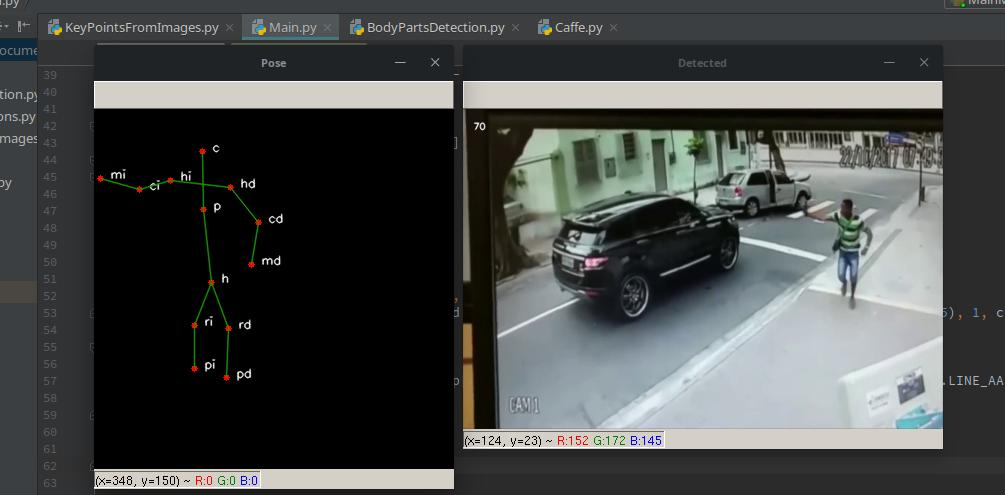
\includegraphics[width=330pt]{Imagenes/results1.jpg}
	\centering	
	\caption{Se visualiza la pose descripta con los puntos de las anotaciones asociadas a la clase de pose (objeto persona) detectada, junto con la imagen original del video en proceso.}
	\label{fig:results1}
\end{figure}	

Los puntos, una vez diagramados en pantalla son unidos por líneas de acuerdo a relaciones de partes preestablecidas: hombros se unen a sus respectivos codos, codos con manos, pies con rodillas, etc.\par

\subsubsection{Conclusión}
El clasificador de objetos dlib entrenado con algunas decenas de imágenes resulta bastante eficiente en términos de velocidad, tomando en cuenta que solamente existen tres clases de poses de aprendizaje. No se agregaron más clases de poses porque ello significaría tiempo de entrenamiento superior al desarrollo del trabajo de tesis.\par

Para verificar el grado de precisión del detector de poses, se hicieron pruebas para:
 \begin{enumerate}
 	\item \textbf{Detectar poses en tiempo real a través de la cámara incorporada al computador:} no detectaba poses humanas teniendo en observación a al menos una persona completa.
 	\item \textbf{Detectar poses en videos descargados de la Internet:} se detectaba un número considerable de falsos positivos, es decir, detectaba poses en donde no existían  humanos en escena.
	\item \textbf{Detectar poses en videos descargados o mediante la cámara incorporada con baja iluminación:} no se detectaban poses humanas bajo condiciones de poca luminosidad escénica en donde, precisamente, existía al menos un cuerpo humano.
\end{enumerate}

Se resolvió descartar un detector de poses usando los módulos de HOG-SVM de la librería dlib debido a que se necesitarían meses de trabajo recopilando imágenes de entrenamiento más nítidas y además calibrar los parámetros necesarios para obtener una precisión aceptable.\par

\subsection{Prueba 2: AlphaPose}
\subsubsection{Descripción}
AlphaPose es un proyecto de estimación precisa de poses humanas en Python que implementa algoritmos basados en el paper de Fang et al. (2018) descrito como Estimación Regional Multipersona.\par

Según la descripción encontrada en github.com, que aloja proyectos de desarrollo a nivel mundial, AlphaPose fue el primer sistema de detección de poses humanas de código abierto.\par

Este sistema utiliza el COCO dataset, que es un conjunto de aproximadamente 80 clases de objetos, 80.000 imágenes de entrenamiento y 40.000 imágenes de validación (ver sitio oficial \url{www.cocodataset.org}).\par

\begin{figure}[h!]
	
\includegraphics[width=250pt]{Imagenes/alphapose.jpg}
	\centering	
	\label{fig:alphapose}
\end{figure}

Además, es compatible con MPII dataset, otro conjunto extenso de imágenes que incluye aproximadamente 25.000 imágenes que contienen cerca de 40.000 anotaciones de cuerpos humanos cubriendo 410 tipos de actividades humanas catalogadas (ver sitio oficial \url{human-pose.mpi-inf.mpg.de}).\par

AlphaPose implementa modelos de CNNs entrenados mediante los dos conjuntos de datos mencionados, haciendo necesario el uso de la tecnología CUDA de nVidia, ya mencionado anteriormente. Afortunadamente, AlphaPose puede correr en computadores que no cuenten con GPUs nVidia omitiendo así el uso de CUDA, aunque esto resulta ser más lento ya que no se cuenta con la característica de multiprocesamiento.\par

Para los resultados, se utilizó código de ejemplo alojado en su página oficial, que permite la ejecución de pruebas para determinar su grado de precisión y velocidad de procesamiento.\par

\subsubsection{Resultados}
Se utilizó código ejemplo oficial de AlphaPose que permite la ejecución de pruebas sin la utilización de GPUs especializados para ejecución en paralelo, lo que resulta conveniente para este trabajo debido a la imposibilidad de contar con una unidad potente de procesamiento. Sin embargo, las pruebas sin GPUs sugirieron una baja tasa de procesamiento de imágenes por segundo (en inglés \textit{Frames Per Second}, o FPS). Ésto sumado a la imposibilidad de cambiar parámetros de la red neuronal embebida, hicieron de este sistema un candidato no utilizable para el entorno con el que se cuenta en este trabajo.\par

La tasa de procesamiento arrojó, en un computador con dos núcleos y sin GPU dedicado, un valor aproximado de 0.066666667 FPS, o lo que es igual, un promedio de 15 segundos de procesamiento por cada imagen. \par

Se aclara, que para las pruebas de las distintas herramientas, se utilizó un único video descargado de Internet, a fin de tener una visión más certera de velocidad al hacer medición sobre un mismo objeto.\par

\subsubsection{Conclusión}
Debido a la baja tasa de procesamiento de AlphaPose sin GPU, se descartó la utilización del mismo para el presente trabajo.\par 

Sin embargo, AlphaPose podría ser utilizado en proyectos que implementen hardware de procesamiento con más potencia, múltiples GPUs y 8 núcleos de procesador como mínimo.\par

\subsection{Prueba 3: Modelo DNN Caffe en OpenCV}
\subsubsection{Descripción}
\textit{Convolutional Architecture for Fast Feature Embedding} (Caffe) en inglés, o Arquitectura convolucional para incrustación rápida de características, es un framework para desarrollo de software enfocado a Machine Learning, desarrollado en la Universidad de Berkeley en California, Jia et al. (2014) explican su desarrollo.\par 

Se trata de un conjunto de librerías C++ para generar modelos, entrenar algoritmos e inferir, utilizando diferentes elementos propios de Machine Learning; también cuenta con una API para Python, según se puede leer en su página web oficial \url{caffe.berkeleyvision.org}.\par 

Existen diferentes modelos de redes neuronales generadas utilizando Caffe en Internet, es así que uno de estos modelos fue creado para la estimación de poses humanas en imágenes. \par

Un modelo de red neuronal consiste en un conjunto de configuraciones para una red previamente entrenada, con sus pesos, capas intermedias y las funciones de entrada, activación y salida correspondientes.\par 

En el sitio web oficial de entrenamiento de OpenCV \url{www.learnopencv.com}, se puede encontrar un modelo Caffe de CNNs utilizado para la estimación de poses humanas, mediante el uso de una red neuronal incluida en las herramientas OpenCV.\par

De esta manera, es posible cargar el modelo preestablecido Caffe utilizando herramientas de redes neuronales profundas embebidas en OpenCV, evitando así, que otro desarrollador pase meses o posiblemente años recopilando información y generando una estructura de red que pueda ser usada por otra persona.\par

En la documentación oficial de OpenCV se pueden encontrar ejemplos de cómo utilizar estos modelos pre entrenados, que, siendo implementados en unas lineas de código Python, permiten estimar poses humanas en imágenes, es así que se desarrolló una aplicación Python para las pruebas. 

\subsubsection{Resultados}
Ejecutar una CNN no es una tarea que requiera pocos recursos, pero a diferencia de las demás pruebas citadas anteriormente, utilizar un modelo preestablecido en OpenCV no requiere de un computador con múltiples GPUs ejecutando CUDA.\par

Sin embargo, implementar las herramientas de CNNs de OpenCV tiene ciertamente una ventaja significativa con respecto a las opciones anteriores: la capacidad de ajustar ciertos parámetros propios de la red, lo que puede incrementar significativamente la velocidad de procesamiento en un computador sin GPU.\par

\subsubsection{Conclusión}
Tomando en cuenta que la velocidad de procesamiento utilizando el modelo Caffe es ligeramente superior a las pruebas anteriores, se optó por utilizarlo para la extracción de poses. Una imagen procesada en un computador con dos núcleos tomó en promedio 8 segundos, sin GPUs para efectuar multiprocesamiento.\par

Aunque es mucho el tiempo necesario para procesar una imagen no lográndose suficiente fluidez para catalogarla como 'en tiempo real', el resultado es bastante acertado, tomando en cuenta las limitaciones del hardware utilizado. Se podría obtener un mejor desempeño usando máquinas más potentes, o simplemente haciendo uso de librerías de paralelismo de Python, que permiten distribuir trabajos no solamente a través de hilos de ejecución, sino también a través de múltiples computadores conectados entre sí por medio de una red de área local.\par

\newpage
\section{Extracción de poses humanas}\label{extraccionpose}
Luego de las pruebas, se decidió utilizar el modelo Caffe mediante la implementación de las funciones DNN de OpenCV. En este apartado se dará una breve explicación de los detalles del mismo.\par

La configuración del modelo de red previamente entrenada se grafica en la siguiente figura:
\begin{figure}[h!]
	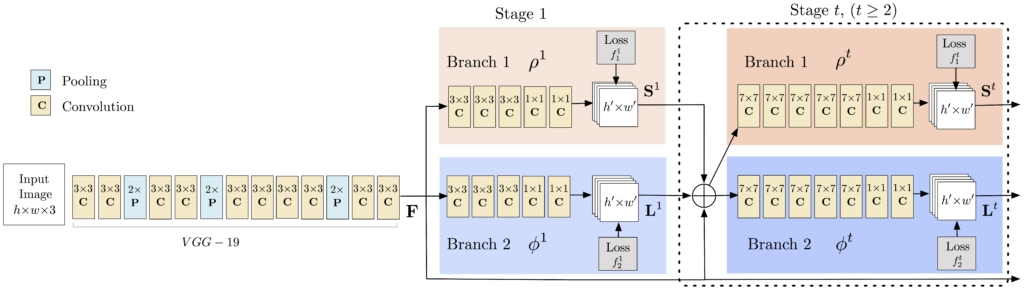
\includegraphics[width=460pt]{Imagenes/network_pose1.jpg}
	\centering	
	\caption{Estructura visual del modelo de red neuronal artificial Caffe para estimación de poses humanas, Fuente \url{learnopencv.com}.}
	\label{fig:network_pose1}
\end{figure}	

Detalles de la estructura:
\begin{enumerate}
	\item Las primeras 10 capas de la red se utilizan para crear un mapa de características de la imagen. Contiene capas pooling y convolucionales.
	\item En la segunda fase (Stage 1), el Branch1 se utiliza para crear un confidence map, en inglés, que es básicamente un mapa de la información ya obtenida. El mapa se realiza en base a las ubicaciones de partes del cuerpo. En el Branch2 se predicen puntos de afinidades, esto es, se trata de predecir a que punto cercano corresponde un punto determinado (ej.: hombro con codo, pie con rodilla, etc.)
	\item En la última fase, se repite una estructura cierta cantidad de veces: se toman los puntos del mapa de afinidades y del mapa de características y se aplica lo que se denomina algoritmo voraz cuya finalidad es elegir la opción óptima dentro de un grupo de alternativas.
\end{enumerate}

El modelo devuelve un conjunto ordenado de puntos que conforman el cuerpo humano comenzando por la cabeza, hasta llegar a los pies. Así, la cabeza tendrá el índice 0 en el arreglo, el cuello será índice 1, hombros 2 y 3, y así sucesivamente hasta llegar a los pies.\par

\section{Cálculo angular de extremidades}\label{calculoangular}

Una vez establecidos los puntos relevantes del cuerpo humano a través de la utilización de una herramienta para la estimación de poses, es necesario establecer los ángulos que las extremidades del cuerpo forman con el tronco del mismo. De ésta manera se puede caracterizar una pose y guardar la configuración de la disposición de los mismos.\par 

Para el cálculo angular, se utilizaron ecuaciones trigonométricas simples como ser: pendiente de una recta, diferencia de pendientes entre dos rectas y distancia existente entre dos puntos en un plano. Del lado derecho del cuerpo, las extremidades inferiores, los ángulos se miden en sentido antihorario tomando como línea de origen el tronco humano, y en sentido horario para las extremidades superiores. Del lado derecho se invierte el sentido, las extremidades superiores tienen sentido antihorario y los inferiores sentido horario.\par

Cada extremidad cuenta con dos partes, teniendo cuatro extremidades, se proceden a calcular ocho ángulos: antebrazos izquierdo y derecho, brazos izquierdo y derecho (sección del músculo biceps), muslos izquierdo y derecho, y pantorrillas izquierda y derecha. Todos estos suman ocho partes a considerar.\par

\begin{figure}[h!]
	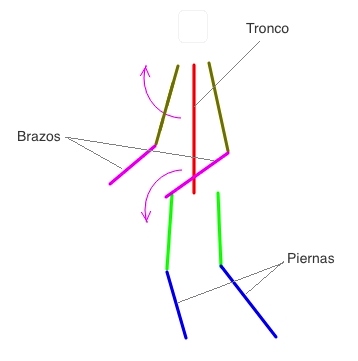
\includegraphics[width=200pt]{Imagenes/pose6.jpg}
	\centering	
	\caption{Ejemplo de medición del lado izquierdo del cuerpo: los miembros superiores, con la flecha que indica el sentido de medición angular, y los inferiores, en sentido contrario. Del lado derecho se invierten los sentidos. Fuente propia.}
	\label{fig:pose5}
\end{figure}

\subsection{Estimación de tronco}
En un escenario perfecto, las imágenes captadas por una cámara pueden describir todas las partes del cuerpo humano de una persona en escena, pero no siempre sucede. Existen ocasiones en que, o el sujeto se encuentra muy cerca de la cámara, o algún objeto se interpone entre el cuerpo y la cámara.\par

El concepto de medición de ángulo entre dos rectas sugiere que ambas deben existir  obligatoriamente, no solamente es necesario que se visualice una extremidad, sino también el tronco del cuerpo humano, que es básicamente el origen de la medición angular en los dos casos citados en la figura. \par

Estimar o suponer la presencia de una extremidad, es más complicado porque no se sabe si la extremidad existe en realidad, o si está dispuesto de una forma que no se puede imaginar o deducir, así que la única opción es intentar estableces la ubicación del tronco, si este no existiese en la imagen.\par

En caso de que no pueda visualizarse el tronco, se siguieron las siguen premisas:
\begin{itemize}
	\item Si los puntos de ambos hombros del cuerpo existen, elegir como ubicación superior del tronco, al punto medio comprendido entre los puntos de los hombros, esto es, utilizando una ecuación trigonométrica, obtener el punto medio entre dos puntos.
	\item Si los puntos de ambas caderas existen, elegir como ubicación inferior del tronco al punto medio comprendido entre ambos puntos.
	\item Si únicamente existe un punto hombro, utilizarlo como ubicación superior, ya que el tronco no se encuentra tan lejos del mismo. Además, esto cubre los casos en que una persona puede no estar mirando a la cámara, y uno de sus hombros es invisible.
	\item Si únicamente existe un punto cadera, utilizarlo como ubicación inferior del tronco, del mismo modo que se utiliza en el ítem anterior para hombro. 
\end{itemize}
	
De esta manera, si no se contaran con los datos explícitos de los puntos que conforman el tronco, es posible deducir su ubicación matemáticamente.\par

\subsection{Representación interna de partes del cuerpo}
Una vez deducido el tronco, se agrupan las ubicaciones de los puntos con sus etiquetas de acuerdo al índice devuelto por el modelo Caffe, y de acuerdo a la categoría de extremidades a la que pertenecen, ejemplo:
\begin{center}
{\footnotesize 'brazoDerecho  ' : [('codoDerecho': (323, 42)),  ('hombroDerecho': (421, 25))]}  \\
{\footnotesize 'piernaIzquierda' : [('pieIzquierdo': (234, 124)), ('rodillaIzquierda': (242, 75))]}\\	
\end{center}

De este modo, se envían como argumentos a una función que obtiene el ángulo entre cada extremidad del cuerpo, con el tronco del mismo, devolviendo un arreglo con la lista de ángulos:
\begin{center}
	{\footnotesize ['brazoDerecho' : 27.3], ['piernaIzquierda' : 12.5]}\\	
\end{center}
Esto se interpreta como: brazoDerecho forma un ángulo de 27.3° con el tronco, piernaIzquierda forma ángulo de 12.5° con el tronco. Esto sucede con las demás extremidades por igual. Al final de todo este proceso, se debe obtener un conjunto de ocho ángulos ordenados para poder ser utilizados como valores individuales de cada entrada de la red neuronal:
\begin{center}
	{\footnotesize [81.2, 41.5, 12.2, 0.0, 155.4, 13.0, 75.3, 43.0]}\\	
\end{center}

\subsection{Generación de datos de entrenamiento}
Se busca ahora generar el conjunto de todos los ángulos posibles para dos clases distintas de poses: poses compatibles con ataque, y poses no compatibles con ataque. La red neuronal debe entrenarse con un mínimo de dos clases para poder devolver una predicción válida, de esta manera, se debe ingresar valores que la red pueda predecir como casos positivos, o de lo contrario, casos negativos.\par

El método de entrenamiento es: se deben generar primero grupos de poses compatibles con agresiones, para el caso de valores positivos, y grupos de poses no compatibles con agresiones, para los negativos.\par

Para el efecto, se procedió a la captura mediante la cámara incorporada del cuerpo humano de una persona en una acción cuya pose sugiera 1. algún tipo de amenaza con arma o 2. agresión con brazos (se podría entrenar con poses de más tipos de agresiones en un trabajo futuro). No se contabilizó el número de casos positivos, ya que simplemente eran almacenados en un archivo. Luego se procedió a la captura de un cuerpo humano cuya pose esté fuera del margen considerado como amenaza o agresión. \par

\begin{table}[htbp]
	\centering
	\footnotesize
	\begin{tabular}{rrcc}
		\raisebox{-\totalheight}{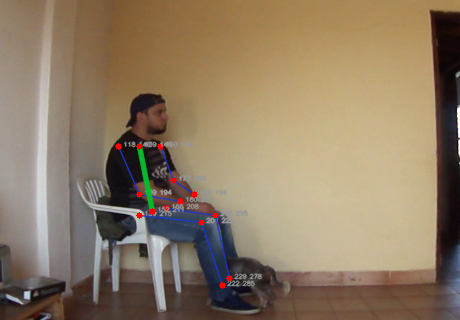
\includegraphics[width=0.25\textwidth]{Imagenes/1.png}} &
		\raisebox{-\totalheight}{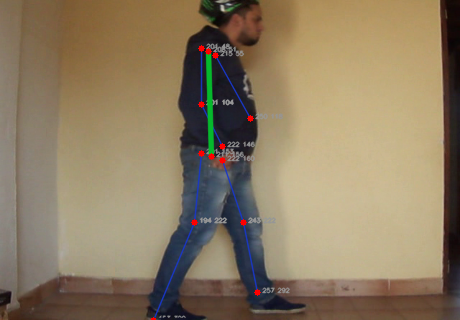
\includegraphics[width=0.25\textwidth]{Imagenes/2.png}} \\ 
		\multicolumn{2}{c}{Negativo para Amenaza/Agresión} \\
		
		\raisebox{-\totalheight}{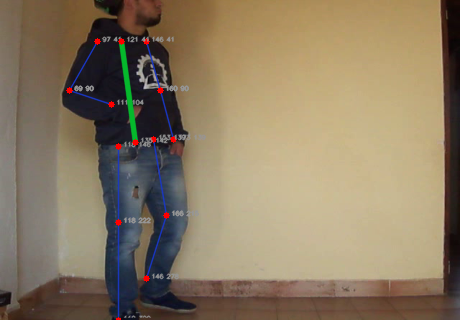
\includegraphics[width=0.25\textwidth]{Imagenes/3.png}} &
		\raisebox{-\totalheight}{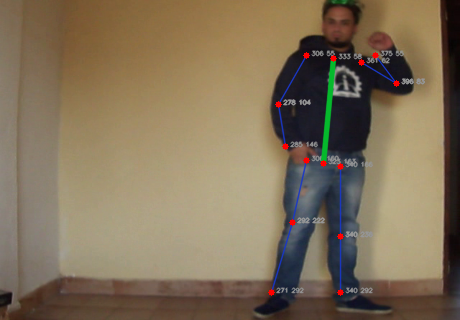
\includegraphics[width=0.25\textwidth]{Imagenes/4.png}} \\
		\multicolumn{2}{c}{Negativo para Amenaza/Agresión} \\
		
		\raisebox{-\totalheight}{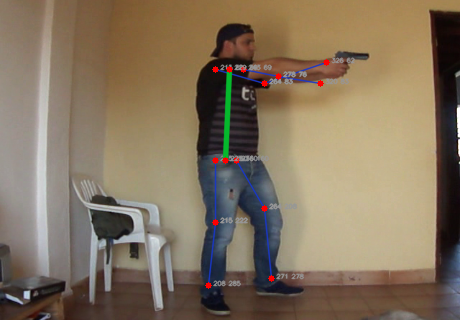
\includegraphics[width=0.25\textwidth]{Imagenes/5.png}} &
		\raisebox{-\totalheight}{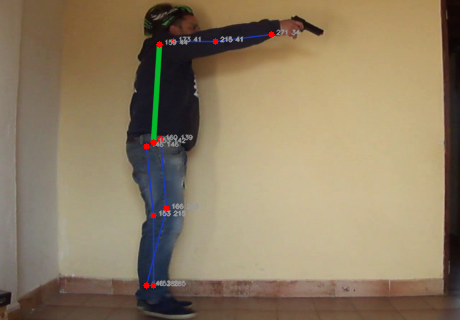
\includegraphics[width=0.25\textwidth]{Imagenes/6.png}} \\ 
		\multicolumn{2}{c}{Positivo para Amenaza/Agresión} \\
	\end{tabular}%
	\label{tab:addlabel}%
	\caption{Tabla de clases de poses utilizadas para entrenamiento.}
\end{table}%


\begin{figure}[h!]
	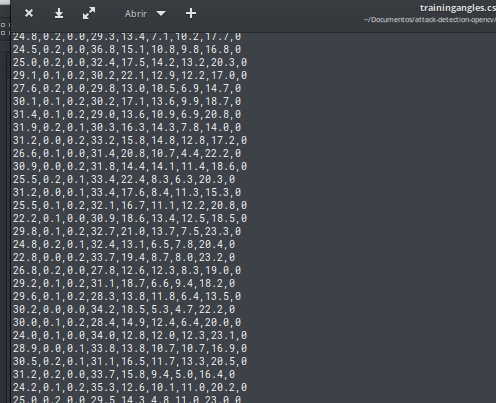
\includegraphics[width=180pt]{Imagenes/dataset2.jpg}
	\centering	
	\caption{Ejemplo de un conjunto de valores de entrenamiento generados.}
	\label{fig:dataset2}
\end{figure}

Se generaron en total 3.246.747 combinaciones de poses positivas y negativas para poses que se utilizarán para entrenar la red neuronal.\par


\section{Entrenamiento de una red neuronal artificial}\label{entrenamiento}
Para la implementación de redes neuronales artificiales en el presente trabajo, se utilizó la librería Keras de Python, que ofrecen una capa de abstracción sobre otra librería llamada TensorFlow.\par

\subsection{Búsqueda de un modelo óptimo}
Los modelos de redes neuronales son variables, y no existe uno preestablecido para la predicción de valores en un problema particular. La búsqueda de un modelo implica la prueba de configuraciones, cambiando el número de capas, el número de neuronas y en algunos casos las funciones de entrada, activación y salida de la red.\par

La finalidad de la búsqueda de un modelo óptimo, es encontrar una configuración de disposición de capas y funciones que reduzcan el margen de error y aumenten la precisión de las predicciones.\par

\subsubsection{Pruebas con modelos de red}
Para determinar el modelo óptimo, se hicieron básicamente 6 pruebas distintas utilizando para la mayoría de los casos 8 entradas (ángulos de la pose), 3 capas en total, 1 neurona en la capa de salida y el optimizador Adam por defecto. Solo en una prueba se utilizaron 4 capas en total.\par

Ya que el optimizador solamente interviene en la etapa de entrenamiento, se decidió no probar con otros optimizadores, el modelo de red resulta sencillo y rápido de inferir.\par

A continuación, se citan las configuraciones de capas y neuronas, y el resultado del valor de precisión obtenido en las pruebas, teniendo en todas ellas una capa de salida.
\begin{itemize}
	\item \textbf{Prueba 1}: 
	Red neuronal con capa de entrada de 14 neuronas, 1 capa oculta de 12 neuronas. Resultado de precisión: 97.7\%.
	\item \textbf{Prueba 2}: 
	Red neuronal con capa de entrada de 12 neuronas, 2 capas ocultas de 14 y 10 neuronas respectivamente. Resultado de precisión: 96.8\%.	
	\item \textbf{Prueba 3}: 
	Red neuronal con capa de entrada de 14 neuronas, 1 capa oculta de 14 neuronas. Resultado de precisión: 97.3\%.	
	\item \textbf{Prueba 4}: 
	Red neuronal con capa de entrada de 14 neuronas, 1 capa oculta de 8 neuronas. Resultado de precisión: 98.4\%.	
	\item \textbf{Prueba 5}: 
	Red neuronal con capa de entrada de 12 neuronas, 1 capa oculta de 10 neuronas. Resultado de precisión: 98.2\%.	
	\item \textbf{Prueba 6}: 
	Red neuronal con capa de entrada de 16 neuronas, 1 capa oculta de 8 neuronas. Resultado de precisión: 99.7\%.	
\end{itemize}

En la figura \ref{fig:results2} se puede observar parte de la información de salida generada durante el entrenamiento de poses en la prueba 6, detallando  el valor de la función pérdida (\textit{loss} en inglés) y la precisión (\textit{accuracy}).

\begin{figure}[h!]
	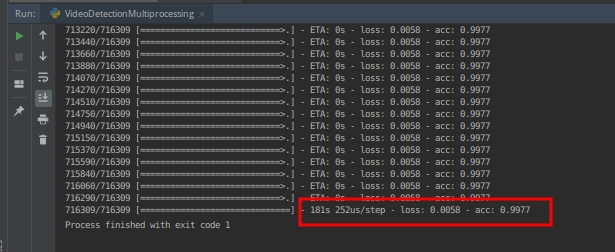
\includegraphics[width=340pt]{Imagenes/results2.jpg}
	\centering	
	\caption{Valores generados en el entrenamiento con poses.}
	\label{fig:results2}
\end{figure}

\textbf{Conclusión:} se decidió por un modelo de 3 capas, detallado en la Prueba 6.

\section{Predicción de poses compatibles con amenazas o agresiones}\label{prediccion}
En este punto, la red entrenada ya está lista para inferir. Al efecto, se escribió una aplicación en Python que puede cargar el modelo pre entrenado de poses, y a medida que va captando imágenes de la cámara incorporada, puede determinar si existe o no una pose compatible con agresión en la imagen.\par


\begin{figure}[h!]
	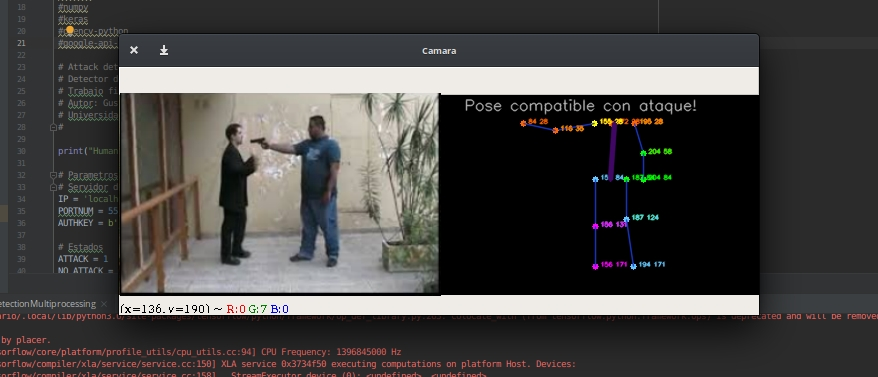
\includegraphics[width=450pt]{Imagenes/output1.jpg}
	\centering	
	\caption{Aplicación ejecutándose, en la que se puede observar un caso positivo para pose compatible con agresión.}
	\label{fig:output1}
\end{figure}

En la ejecución esto va acompañado de una alerta sonora avisando de la detección de una pose compatible, una alerta visual con un mensaje, y se agregó otra alerta visual donde se muestra un círculo rojo en caso de presencia de armas de fuego cortas.\par

\section{Detección de armas utilizando clasificadores en cascada}\label{deteccionarmas}
Si bien la aplicación puede determinar mediante redes neuronales la ocurrencia de una pose compatible con una agresión, también se agregó una característica que permite detectar armas de fuego en la mano de la persona cuya pose resultó positiva para la clasificación.\par

\begin{figure}[h!]
	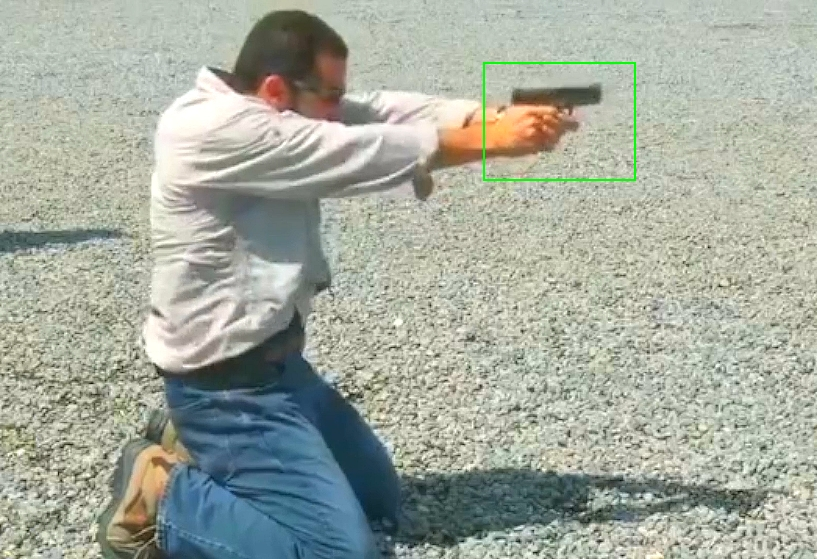
\includegraphics[width=190pt]{Imagenes/output2.jpg}
	\centering	
	\caption{Detección de armas de fuego cortas en la mano de una persona cuya pose es compatible con una amenaza..}
	\label{fig:output2}
\end{figure}

Para el trabajo, se descargó un conjunto de datos pre entrenados de \url{https://github.com/JYang25/opencv_demo} que contiene características de features Haar-like que describen armas de fuego.\par

Para determinar si una agresión con arma de fuego está ocurriendo, además de una pose compatible, es necesario determinar la existencia del objeto arma en la escena, y ésta debe estar situada en una posición que sugiera que una persona la esté utilizando. \par

Un arma en la escena no es determinante para establecer que existe una amenaza, debemos descartar, por ejemplo, armas tiradas en el suelo, colgadas en la pared, o incluso un arma visible en el bolsillo de una persona. Entonces, dos condiciones son necesarias para establecer una amenaza con arma de fuego: una pose compatible con amenaza, y un arma en la mano de la persona.\par

La detección se efectúa mediante Clasificadores en Cascada, cuyo funcionamiento ya se explicó en la sección \ref{herramientasdevisionporcomputadora}, que por defecto se implementan en OpenCV. El proceso de detección de armas se activa luego de que una pose compatible con agresión es detectada, y solamente se genera una alerta extra en caso de que el arma esté ubicada cerca de los puntos de la mano de aquella pose positiva para agresión.\par

No se incluyeron datos de características de todas las armas disponibles para efectuar agresiones humanas (cuchillos, hachas, arcos y flechas, etc), solamente fueron utilizados descriptores de armas de fuego cortas.\par

\vspace*{1cm}

\begin{figure}[h!]
	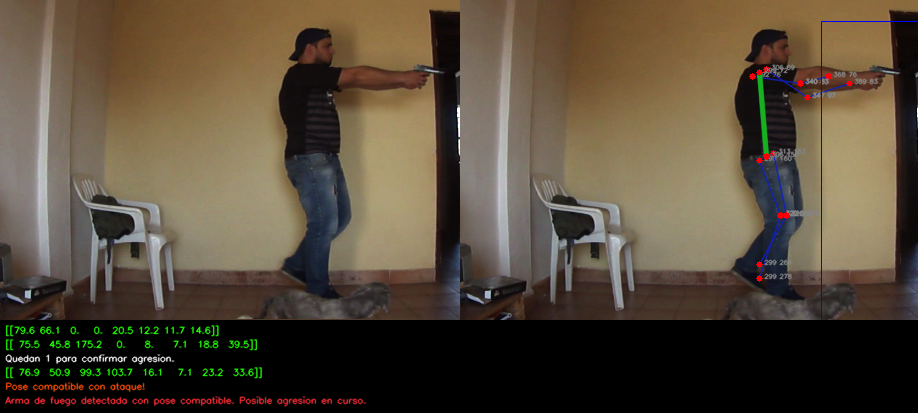
\includegraphics[width=450pt]{Imagenes/positiveresult.jpg}
	\centering	
	\caption{Captura, clasificación y detección de arma positivas para una pose compatible con agresión. Nótese el recuadro de color azul rodendo el área donde se detecta el arma de fuego.}
	\label{fig:code1}
\end{figure}

\section{Esquema de proceso}\label{processschema}
La aplicación desarrollada procesa la información siguiendo la estructura de procesamiento distribuído tipo cliente-servidor que posibilita la modularización. Una estructura cliente-servidor es un modelo de trabajo flexible donde el cliente puede ejecutarse en una computadora dedicada, conectada al servidor a través de una red de área local. Además, esto posibilita que el cliente, al ejecutarse independientemente del servidor, pueda utilizar cualquier herramienta de extracción de poses existente que se quiera implementar. \par

De esta manera, el servidor solamente envía al cliente datos de imágenes, el cliente (o clientes) procesa la información y devuelve al servidor una lista de ángulos de poses, si existiesen. El servidor, al recibir esto, utiliza los datos para entradas en la red neuronal, que determina si el conjunto de ángulos es o no compatible con una pose de agresión.\par

\vspace*{0.7cm}

\begin{figure}[h!]
	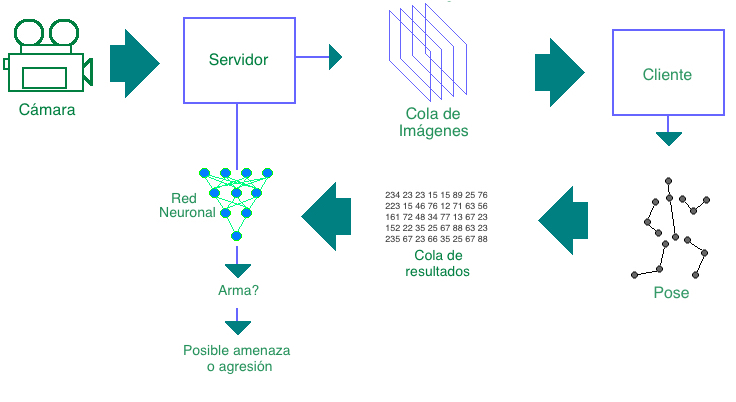
\includegraphics[width=460pt]{Imagenes/process1.jpg}
	\centering	
	\caption{Esquema gráfico del proceso completo. Fuente propia.}
	\label{fig:code1}
\end{figure}

Entonces, citando detalladamente los pasos del proceso, tenemos que:
\begin{enumerate}
	\item La cámara captura imágenes y las envía al servidor.
	\item El servidor recibe las imágenes y las coloca en una cola de procesamiento para las aplicaciones clientes.
	\item Una aplicación cliente lee la imágen existente en la cola y la procesa con el detector de poses implementado.
	\item El detector de poses del cliente obtiene los puntos pertenecientes a las articulaciones del cuerpo humano, si existiese en la imágen, y calcula los ángulos entre rectas de las extremidades con la recta trazada a través del tronco del cuerpo.
	\item El cliente envía a una cola de resultados la lista de ángulos obtenidos de la pose.
	\item El servidor lee datos de la cola de resultados, y utiliza estos como datos de entrada para una red neuronal que clasificará al conjunto de ángulos como compatibles con amenaza, o no compatibles.
	\item Si el resultado de la inferencia de la red neuronal resulta en positiva para pose compatible con amenaza, se procesa la imágen para determinar si existe un objeto arma presente en cercanías a los puntos pertenecientes a las manos de la persona cuya pose se procesó previamente.
	\item Se informa al usuario acerca del resultado de los procesos. Si la pose es compatible o no, y si existe o no un arma de fuego presente en caso de pose positiva.
	\item Se repite el proceso con cada imágen recibida de la cámara.
	\item Se utiliza un algoritmo para descartar falsos positivos: deben existir al menos \textit{x} poses sucesivas compatibles con agresión en \textit{y} segundos. Estos parámetros son ajustables de acuerdo a la velocidad de procesamiento de los clientes. Generalmente los falsos positivos son únicos, no consecutivos en un determinado período de tiempo.
\end{enumerate}\par

\newpage
\chapter{Resultados}
\section{Resumen de resultados de clasificación}\label{results1}
Se utilizó un modelo de red neuronal entrenada con combinaciones de medidas angulares para obtener la clasificación de dos clases: Ataque o no ataque. 

\subsection{Muestras utilizadas}
En esta sección, se considera positiva la pose que sugiera efectivamente que una persona está profiriendo una amenaza o agresión, de lo contrario, se considera negativa.
\begin{itemize}
	\item Amenaza o agresión positiva.
	Para los casos donde la clasificación de la red neuronal sea positiva para Ataque, se utilizaron dos tipos de combinaciones de poses:
	\begin{enumerate}
		\item Ataque o agresión con brazos por sobre la cabeza.
		\item Ataque o agresión con brazos extendidos formando ángulos con el cuerpo cercanos a los 90 grados (amenaza con arma de fuego).
	\end{enumerate}\par
	\item Amenaza o agresión negativa.
	Para casos donde la pose no es considerada como compatible con agresión, se utilizaron combinaciones de ángulos de poses de:
	\begin{enumerate}
		\item Persona caminando.
		\item Persona sentada con brazos en distintas combinaciones angulares cercanas a cero grados (brazos caídos).
		\item Persona de pie con brazos cruzados o a la cintura.
	\end{enumerate}\par	
\end{itemize}\par

\subsection{Tablas de resultados}
Para la siguiente tabla, se utilizó un video en cuyas imágenes el actor efectúa poses negativas y positivas para agresiones/amenazas, obteniendo:

\vspace*{0.8cm}
% Table generated by Excel2LaTeX from sheet 'Resultados'
\begin{table}[htbp]
	\tiny
	\centering
	\resizebox{\textwidth}{!}{% 
		\begin{tabular}{lcccccc}
			\textcolor[rgb]{ .255,  .243,  .212}{} & \multicolumn{1}{p{4.355em}}{\cellcolor[rgb]{ .784,  .941,  .984}\textcolor[rgb]{ .255,  .243,  .212}{\textbf{Tiempo de video en segs}}} & \multicolumn{1}{p{3em}}{\cellcolor[rgb]{ .784,  .941,  .984}\textcolor[rgb]{ .255,  .243,  .212}{\textbf{Total poses}}} & \multicolumn{1}{p{3.285em}}{\cellcolor[rgb]{ .784,  .941,  .984}\textcolor[rgb]{ .255,  .243,  .212}{\textbf{Falsos positivos}}} & \multicolumn{1}{p{3.57em}}{\cellcolor[rgb]{ .784,  .941,  .984}\textcolor[rgb]{ .255,  .243,  .212}{\textbf{Verdaderos positivos}}} & \multicolumn{1}{p{4.215em}}{\cellcolor[rgb]{ .784,  .941,  .984}\textcolor[rgb]{ .255,  .243,  .212}{\centering \textbf{Porcent. de aciertos}}} & \multicolumn{1}{p{3.715em}}{\cellcolor[rgb]{ .784,  .941,  .984}\textcolor[rgb]{ .255,  .243,  .212}{\centering \textbf{Porcent. de errores}}} \\[6ex]
			\textcolor[rgb]{ .255,  .243,  .212}{\textbf{Poses negativas}} & \textcolor[rgb]{ .255,  .243,  .212}{\textbf{64}} & \textcolor[rgb]{ .255,  .243,  .212}{\textbf{1611}} & \textcolor[rgb]{ .255,  .243,  .212}{\textbf{95}} & \textcolor[rgb]{ .255,  .243,  .212}{\textbf{1516}} & \textcolor[rgb]{ .255,  .243,  .212}{\textbf{94.10}} & \textcolor[rgb]{ .255,  .243,  .212}{\textbf{5.90}} \\[1ex]
			\textcolor[rgb]{ .255,  .243,  .212}{\textbf{Poses positivas}} & \textcolor[rgb]{ .255,  .243,  .212}{\textbf{31}} & \textcolor[rgb]{ .255,  .243,  .212}{\textbf{795}} & \textcolor[rgb]{ .255,  .243,  .212}{\textbf{81}} & \textcolor[rgb]{ .255,  .243,  .212}{\textbf{714}} & \textcolor[rgb]{ .255,  .243,  .212}{\textbf{89.81}} & \textcolor[rgb]{ .255,  .243,  .212}{\textbf{10.19}} \\[1ex]
			\rowcolor[rgb]{ .827,  .953,  .988} \textcolor[rgb]{ .255,  .243,  .212}{\textbf{Total}} & \textcolor[rgb]{ .255,  .243,  .212}{\textbf{96}} & \textcolor[rgb]{ .255,  .243,  .212}{\textbf{2406}} & \textcolor[rgb]{ .255,  .243,  .212}{\textbf{176}} & \textcolor[rgb]{ .255,  .243,  .212}{\textbf{2230}} & \textcolor[rgb]{ .255,  .243,  .212}{\textbf{92.68}} & \textcolor[rgb]{ .255,  .243,  .212}{\textbf{7.32}} \\
		\end{tabular}%
	}
	\label{tab:addlabel}%
	\caption{Tabla de resultados de pruebas finales obtenidas con la red neuronal. }
\end{table}%
\vspace*{0.1cm}

Del análisis de los datos expuestos en la tabla de resultados, se comprueba que de un total de 2406 imágenes de poses tomadas de un video de prueba, se obtuvieron 2230 casos de clasificación exitosos donde la pose se considera positiva o negativa para agresiones, y 176 casos no exitosos, donde la clase obtenida por la red neuronal no coincidía con las poses de agresión o no agresión. Esto da un valor de precisión de 0,92.\par

De los datos obtenidos, se puede construir una matriz de confusión como sigue:\par
\vspace*{1cm}
% Table generated by Excel2LaTeX from sheet 'Confusion'
\begin{table}[htbp]
	\centering
	\footnotesize
	\begin{tabular}{rrcc}
		\rowcolor[rgb]{ .827,  .953,  .988} \textcolor[rgb]{ .729,  .71,  .671}{} & \multicolumn{3}{c}{\cellcolor[rgb]{ .886,  .984,  .984}\textcolor[rgb]{ .729,  .71,  .671}{\textbf{Prediccion}}} \\[1ex]
		\rowcolor[rgb]{ .827,  .953,  .988} \textcolor[rgb]{ .729,  .71,  .671}{} & \textcolor[rgb]{ .255,  .243,  .212}{} & \multicolumn{1}{p{5.355em}}{\cellcolor[rgb]{ .784,  .941,  .984}\textcolor[rgb]{ .255,  .243,  .212}{\textbf{Poses Positivas}}} & \multicolumn{1}{p{5.355em}}{\cellcolor[rgb]{ .784,  .941,  .984}\textcolor[rgb]{ .255,  .243,  .212}{\textbf{Poses Negativas}}} \\[2ex]
		\rowcolor[rgb]{ .827,  .953,  .988} \multicolumn{1}{c}{\multirow{2}[0]{*}{\textcolor[rgb]{ .729,  .71,  .671}{\rotatebox{90}{\textbf{Real}}}}} & \multicolumn{1}{l}{\textcolor[rgb]{ .255,  .243,  .212}{\textbf{Poses Positivas}}} & \cellcolor[rgb]{ 1,  1,  1}\textcolor[rgb]{ .255,  .243,  .212}{\textbf{714}} & \cellcolor[rgb]{ 1,  1,  1}\textcolor[rgb]{ .255,  .243,  .212}{\textbf{81}} \\[2ex]
		\rowcolor[rgb]{ .827,  .953,  .988}       & \multicolumn{1}{l}{\textcolor[rgb]{ .255,  .243,  .212}{\textbf{Poses Negativas}}} & \cellcolor[rgb]{ 1,  1,  1}\textcolor[rgb]{ .255,  .243,  .212}{\textbf{95}} & \cellcolor[rgb]{ 1,  1,  1}\textcolor[rgb]{ .255,  .243,  .212}{\textbf{1516}} \\[2ex]
		\rowcolor[rgb]{ .827,  .953,  .988}       & \textcolor[rgb]{ .255,  .243,  .212}{} & \textcolor[rgb]{ .255,  .243,  .212}{\textbf{Exactitud}} & \textcolor[rgb]{ .255,  .243,  .212}{\textbf{Presición}} \\[1ex]
		\rowcolor[rgb]{ .827,  .953,  .988}  	  & \textcolor[rgb]{ .729,  .71,  .671}{} & \cellcolor[rgb]{ 1,  1,  1}\textcolor[rgb]{.255,  .243,  .212}{\textbf{0.94}} & \cellcolor[rgb]{ 1,  1,  1}\textcolor[rgb]{.255,  .243,  .212}{\textbf{0.93}} \\[1ex]
	\end{tabular}%
	\caption{Matriz de confusión generada con los datos de las pruebas finales.}
	\label{tab:addlabel}%
\end{table}%


\newpage
\chapter{Conclusiones}
A través del trabajo desarrollado, se evidencia el cumplimiento del objetivo general que consiste en desarrollar una solución computacional que permite la detección básica de agresiones o amenazas humanas, mediante el entrenamiento de redes neuronales de computadoras.\par

Estudiada la pose expresada por la disposición de las extremidades de una persona, con aplicación de conceptos y técnicas de Machine Learning a través de redes neuronales, y los principios de Visión por Computadora, se desarrolló el software que logra la detección de poses consideradas como amenazas o agresiones a través del análisis de imágenes en las que se efectúa el cálculo angular de las líneas formadas por las extremidades y el tronco.\par

Se logró desarrollar una aplicación que aporta una solución para la detección de agresiones humanas en imágenes secuenciales capturadas en videos, sin armas o con armas de fuego cortas.\par

\chapter{Trabajos a futuro}
\begin{itemize}
	\item Utilización de múltiples fuentes (cámaras) para la recolección de imágenes haciendo de la aplicación una herramienta de detección completa en entornos visuales más amplios (ejemplo: plazas, locales de reunión, y otros lugares públicos).\par

	\item Considerar agresiones incluyendo una mayor cantidad de tipos de armas que puedan ser utilizadas por el humano para proferir agresiones.\par

	\item Implementar un detector de poses mediante redes neuronales convolucionales que no requieran el uso de GPUs.\par
\end{itemize}

\newpage
\chapter{Glosario de Términos}
\setlength{\parskip}{-1.0em}
\setlength{\parindent}{0em}
 
\textbf{AI} Artificial Intelligence, en inglés. Inteligencia Artificial en castellano. Es la ciencia que estudia la simulación de procesos y comportamiento del cerebro humano aplicados a la informática.\\
 
\textbf{Algoritmo} Conjunto de instrucciones o reglas , ordenadas que permiten llevar a cabo una actividad mediante pasos sucesivos, con inicio y fin.\\
 
\textbf{ASIP} Siglas en inglés de Application-Specific Information Processing, que significa Procesamiento de Información Específica de Aplicación.\\
 
\textbf{Backpropagation} En ingles.  Significa Propagación hacia atrás, es un algoritmo de ajuste de pesos de redes neuronales.\\

\textbf{Caffe} Siglas en inglés de Convolutional Architecture for Fast Feature Embedding, es un framwork enfocado a Machine Learning.\\
 
\textbf{CCTV} Siglas de Circuito Cerrado de TeleVisión, sistema de cámaras interconectadas para el monitoreo remoto.\\
 
\textbf{Clasificador} Un clasificador es un proceso algorítmico capaz de identificar objetos de cierta clase de un conjunto universo de objetos.\\
 
\textbf{Clasificador Lineal} Clasificador cuyas clases de objetos son perfectamente separables a través de una línea recta.\\
 
\textbf{Clasificador Multiclase} Refiere a un tipo de clasificador que puede identificar más de un tipo de objeto de un conjunto.\\
 
\textbf{CNN} En iglés, siglas de Convolutional Neural Network. Redes neuronales convolucionales, son redes especiales para predicción en imágenes.\\
 
\textbf{CUDA} Siglas en inglés de Compute Unified Device Architecture, traducido sería Arquitectura Unificada de Dispositivos de Cómputo. Es una interfaz de programación paralela para dispositivos gráficos marca nVidia.\\
 
\textbf{Dataset} Es el término en inglés que se refiere a un conjunto de datos agrupados para cierto propósito. Ej.: dataset de entrenamiento.\\
 
\textbf{DNN} Siglas en inglés de Deep Neural Network. Redes neuronales profundas, de múltiples capas.\\
 
\textbf{DVR} Siglas en inglés de Digital Video Recorder. Dispositivo digital capaz de capturar, almacenar y procesar imágenes a través de cámaras de vigilancia. Es el sucesor de los VCRs.\\
 t
\textbf{Feature} Palabra en inglés que hace referencia a una clase de característica de entrada en un clasificador. El conjunto de features es el conjunto de características. Cada feature representa una característica del conjunto.\\
 
\textbf{Framework} Palabra en inglés que significa Marco de trabajo, es un conjunto de librerías de código empaquetadas que contienen funciones y procedimientos con un nivel de abstracción mayor.\\
 
\textbf{Función Kernel} O función núcleo, en Inteligencia Artificial es una función matemáticas utilizada para proyectar datos en un plano a través de una nueva dimensión.\\
 
\textbf{Función objetivo} Función lineal de varias variables, cuyo valor es maximizable o minimizable.  Utilizada generalmente en problemas de optimización.\\
 
\textbf{Gaussian} Refiere a la función Gaussiana, utilizada en estadísticas como una función de densidad de la distribución normal.\\
 
\textbf{GPU} Graphic Process Unit en inglés, se denominan así a las tarjetas aceleradoras de gráficas de las computadoras.\\
 
\textbf{Gradiente} Vector en análisis matemático que indica la medida en la cual una variable cambia de manera rápida su valor, y la dirección de cambio.\\
 
\textbf{Haar-like Features} Datos de entrada de un clasificador en cascada que representan ciertas disposiciones específicas de pixeles de una imagen.\\
 
\textbf{Hiperplano} En el  plano cartesiano, un hiperplano es una recta que divide el plano en dos mitades. Es una recta de separación.\\
 
\textbf{Histograma} Representación gráfica de una variable en forma de barras, cada barra representa la proporción de la frecuencia de los valores.\\
 
\textbf{IA} Inteligencia Artificial.\\
 
\textbf{Keras} Librería de código abierto para inteligencia artificial escrita en Python, provee una capa de abstracción sobre otras librerías como Tensorflow.\\
 
\textbf{Machine Learning} En inglés, traducción literal sería Aprendizaje de la máquina. Ciencia relacionada a la Inteligencia Artificial que intenta simular el razonamiento del cerebro humano en computadoras mediante algoritmos, funciones matemáticas y probabilidades.\\
 
\textbf{nVidia} Corporación internacional que fabrica y distribuye componentes de computadoras dedicados al procesamiento gráfico.\\
 
\textbf{OpenCV} Open Computer Vision en inglés, es una librería de funciones y procedimientos escrita para el procesamiento de imágenes por computadora\\
 
\textbf{PC} Personal Computar, en inglés. Computadora personal. Término abreviado para referirse normalmente a un computador.\\
 
\textbf{Pedestrian Detection} Traducción del inglés que significa Detección de peatones.\\
\textbf{Pixel} Unidad mínima de datos en una imagen. Un pixel representa color e intensidad en un punto de la imagen.\\
 
\textbf{Polinomial} Función con estructura de polinomio.\\
 
\textbf{POO} Siglas de Programación Orientada a Objetos cuya filosofía se basa en la representación de entidades como si fueran objetos de la vida real.\\
 
\textbf{Raspberry Pi} Dispositivo programable de licencia abierta para proyectos electrónicos.\\
 
\textbf{RNA} Siglas de Redes Neuronales Artificiales.\\

\textbf{Sigmoidea} Función que describe una curva con progresión temporal, desde niveles bajos a altos, cuya transición se acelera cuando el valor X se acerca a 0.\\

\textbf{Software} Acrónimo en inglés acuñado al término informático que describe a un programa o conjunto de ellos.\\

\textbf{Support Vector Machines (SVM)} Traducción al inglés de Máquinas de Vectores Soporte. Técnica de clasificación que utiliza hiperplanos para separar la información.\\

\textbf{Tensorflow} Librería de código abierto para Python creada por Google, para Inteligencia Artificial.\\

\textbf{VCR} En inglés, siglas de Video Camera Recorder. Es un dispositivo analógico que permite capturar las imágenes a través de cámaras de vigilancia. \\


\newpage	
\chapter{Referencias}
\setlength{\parskip}{3em}
\setlength{\parindent}{0em}
\begin{enumerate}
	\item M. Valera, S.A. Velastin. \textit{Intelligent distributed surveillance system: a review. IEE Proc. Vis. Image Signal Process.} 152(3):192–204, 2005.
	
	\item R. Dautov, S. Distefano, D. Bruneo, F. Longo, G. Merlino, A. Puliafito, R. Buyya. \textit{Metropolitan intelligent surveillance systems for urban areas by harnessing IoT and edge computing paradigms.} 48(2):1475–1492, 2018.

	\item M. D. Ruiz Lozano. \textit{Un modelo para el desarrollo de sistemas de detección de situaciones de riesgo capaces de integrar información de fuentes heterogéneas. Aplicaciones.} Granada, 2010.

	\item Zhang, G.D., Jiang, P.L., Matsumoto, K., Yoshida, M. and Kita, K. \textit{An Improvement of Pedestrian Detection Method with Multiple Resolutions.} Journal of Computer and Communications. 5(1) 102-116, 2017.

	\item Nidhi. Dept. of Computer Applications, NIT Kurukshetra, Haryana, India. \textit{Image Processing and Object Detection.} International Journal of Applied Research 2015; 1(9): 396-399, 2015.
	
	\item J.L. Barron, D.J. Fleet, S.S. Beauchemin. \textit{Performance of Optical Flow Techniques.} IJCV 12:1 pp43-77, 2015.
	
	\item N. S. Kamarudin, M. Makhtar, S. A. Fadzli, M. Mohamad, F. S. Mohamad, M. F. A. Kadir. \textit{Comparison of Image Classification Techniques using Caltech 101 Dataset.} Journal of Theoretical and Applied Information Technology, 71(2):1992-8645, 2015.
	
	\item S. Bailey, C. Aragon, R. Romano, R. C. Thomas, B. A. Weaver, D. Wong. \textit{How to find more Supernovae with less work: Object Classification Techniques for Difference Imaging.} Journal of Theoretical and Applied Information Technology, 665(2):1246-1253, 2007.
	
	\item Intel Corp. \textit{The OpenCV Reference Manual, Release 3.0.0-dev} 2014. 
			
	\item Andrew Ng. \textit{Machine Learning Course}, Coursera, www.coursera.org. 
	
	\item Damián Jorge Matich. \textit{Redes Neuronales: Conceptos Básicos y Aplicaciones}, Universidad Tecnológica Nacional, 2001. 
	
	\item C.Enyinna Nwankpa, W. Ijomah, A. Gachagan, and S. Marshall. \textit{Activation Functions: Comparison of Trends in Practice and Research for Deep Learning}, 2018.
	
	\item Enrique J. Carmona Suárez. \textit{Tutorial sobre Máquinas de Vectores Soporte (SVM)}, Universidad Nacional de Educación a Distancia (UNED), 28040-Madrid España, 2014.
	
	\item N. Dalal, B. Trigg. \textit{Histograms of Oriented Gradients for Human Detection}, EEE Computer Society Conference on Computer Vision and Pattern Recognition, (1):886–893, 2005.
	
	\item Ong Chin Ann, Lau Bee Theng. \textit{Human Activity Recognition: A Review}, 2014 IEEE International Conference on Control System, Computing and Engineering, 2014.
	
	\item Joan Reig Doménech. \textit{Estudio del estado del arte de los métodos de estimación de la pose humana en 3D}, Universidad de Alicante, España, 2018.
	
	\item H.Fang, S.Xie, Y.Tai, C.Lu. \textit{RMPE: Regional Multi-Person Pose Estimation}, Shanghai Jiao Tong University, China, 2018.
	
	\item Y.LeCun, L.Bottou, Y.Bengio, P.Haffner. \textit{Gradient-Based Learning Applied to Document Recognition}, IEEE, 1998.
	
	\item Z.Cao, T.Simon, S.Wei, Y.Sheikh. \textit{Realtime Multi-Person 2D Pose Estimation using Part Affinity Fields}, The Robotics Institute, Carnegie Mellon University, 2017.

	\item Jia, Yangqing and Shelhamer, Evan and Donahue, Jeff and Karayev, Sergey and Long, Jonathan and Girshick, Ross and Guadarrama, Sergio and Darrell, Trevor. \textit{Caffe: Convolutional Architecture for Fast Feature Embedding}, arXiv preprint arXiv:1408.5093, 2014.
	
	\item Stephen Marsland. \textit{Chapman \& Hall/CRC Machine Learning An Algorithmic Perspective Second Edition}, CRC Press, 2014.
	
	\item Diccionario en línea de la Real Academia Española. \textit{Real Academia Española}. https://dle.rae.es/.
	
	\item J. K. Aggarwal, M. S. Ryoo. \textit{Human Activity Analysis: A Review}, ACM Comput. Surv. 43, 3, Article 16. 2011.
	
	\item T.Subetha, S.Chitrakala. \textit{A Survey on Human Activity Recognition from Videos}, International Conference On Information Communication And Embedded System (ICICES), 2016.
\end{enumerate}
\end{document}